\documentclass[t,aspectratio=169]{beamer}
\usepackage{physics}
\usepackage{amsmath}
\usepackage{tikz}
\usepackage{mathdots}
\usepackage{yhmath}
\usepackage{cancel}
\usepackage{color}
\usepackage{siunitx}
\usepackage{array}
\usepackage{multirow}
\usepackage[version=4]{mhchem}
\usepackage{amssymb}
\usepackage{textcomp, gensymb}
\usepackage{mathtools}
\usepackage{pifont}
\newcommand{\cmark}{\ding{51}}%
\newcommand{\xmark}{\ding{55}}%
\usepackage{fontawesome5}
\usepackage{tabularx}
\usepackage{extarrows}
\usepackage{booktabs}
\usetikzlibrary{fadings}
\usetikzlibrary{patterns}
\usetikzlibrary{shadows.blur}
\usetikzlibrary{shapes}
\usepackage[style=authoryear,backend=bibtex]{biblatex}
\addbibresource{gw.bib}
\renewcommand{\footnotesize}{\scriptsize}
\usepackage{listings}
\usepackage{hyperref}

\newcommand{\pair}[1]{\langle #1 \rangle}
\DeclareMathOperator{\ee}{e}
\DeclareMathOperator{\ii}{i}
\DeclareMathOperator{\sgn}{sgn}

\newcommand{\concept}[1]{\textbf{#1}}
\newcommand*{\abinitio}{\textit{ab initio}}
\newcommand{\shortcode}[1]{\texttt{#1}}
\newcommand*{\const}{\text{const}}

%region Theme 

\usetheme{metropolis}

% Show section in foot
\makeatletter
\setbeamertemplate{footline}
{
  \leavevmode%
  \hbox{%
  \begin{beamercolorbox}[wd=.333333\paperwidth,ht=2.25ex,dp=1ex,center]{author in head/foot}%
    \usebeamerfont{author in head/foot}\insertauthor
  \end{beamercolorbox}%
  \begin{beamercolorbox}[wd=.333333\paperwidth,ht=2.25ex,dp=1ex,center]{title in head/foot}%
    \usebeamerfont{title in head/foot}\insertsection
  \end{beamercolorbox}%
  \begin{beamercolorbox}[wd=.333333\paperwidth,ht=2.25ex,dp=1ex,right]{date in head/foot}%
    \usebeamerfont{date in head/foot}\insertshortdate{}\hspace*{2em}
    \insertframenumber{} / \inserttotalframenumber\hspace*{2ex} 
  \end{beamercolorbox}}%
  \vskip0pt%
}
\makeatother

%endregion

%region  Disable unsupported commands in bookmark titles 
\pdfstringdefDisableCommands{%
  \def\\{}%
  \def\texttt#1{<#1>}%
  \def\mathbb#1{#1}%
}
\pdfstringdefDisableCommands{\def\eqref#1{(\ref{#1})}}

\makeatletter
\pdfstringdefDisableCommands{\let\HyPsd@CatcodeWarning\@gobble}
\makeatother

%endregion

%Remove navigation symbols
\setbeamertemplate{navigation symbols}{}
%Remove frame continuation numbering
\setbeamertemplate{frametitle continuation}{}


%Information to be included in the title page:
\title{Why \shortcode{pseudobands} works?}
\subtitle{Numerical experiments, analysis, and possible enhancement of the method}
\author{Jinyuan Wu}

\begin{document}

\maketitle


\section{A review of $GW$}

\begin{frame}[allowframebreaks]
\frametitle{$GW$ in momentum space}

$- \ii \Sigma \approx GW^{\text{RPA}} = \begin{gathered}
    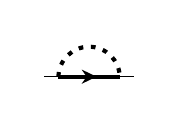
\begin{tikzpicture}[x=0.75pt,y=0.75pt,yscale=-0.65,xscale=0.65, baseline=(XXXX.south) ]
    \path (0,57);\path (87.33333587646484,0);\draw    ($(current bounding box.center)+(0,0.3em)$) node [anchor=south] (XXXX) {};
    %Straight Lines [id:da4779610823231175] 
    \draw [color={rgb, 255:red, 0; green, 0; blue, 0 }  ,draw opacity=1 ]   (12.33,36.33) -- (22.78,36.33) ;
    %Straight Lines [id:da9873503675232067] 
    \draw [color={rgb, 255:red, 0; green, 0; blue, 0 }  ,draw opacity=1 ]   (68.1,36.33) -- (78.55,36.33) ;
    %Straight Lines [id:da09313351721820862] 
    \draw [color={rgb, 255:red, 0; green, 0; blue, 0 }  ,draw opacity=1 ][line width=1.5]    (22.78,36.33) -- (68.1,36.33) ;
    \draw [shift={(51.04,36.33)}, rotate = 180] [fill={rgb, 255:red, 0; green, 0; blue, 0 }  ,fill opacity=1 ][line width=0.08]  [draw opacity=0] (11.07,-5.32) -- (0,0) -- (11.07,5.32) -- (7.35,0) -- cycle    ;
    %Shape: Arc [id:dp7767262671888671] 
    \draw  [draw opacity=0][dash pattern={on 1.69pt off 2.76pt}][line width=1.5]  (22.78,36.33) .. controls (23.05,23.96) and (33.2,14.05) .. (45.62,14.11) .. controls (58.08,14.17) and (68.16,24.25) .. (68.24,36.67) -- (45.51,36.84) -- cycle ; \draw  [color={rgb, 255:red, 0; green, 0; blue, 0 }  ,draw opacity=1 ][dash pattern={on 1.69pt off 2.76pt}][line width=1.5]  (22.78,36.33) .. controls (23.05,23.96) and (33.2,14.05) .. (45.62,14.11) .. controls (58.08,14.17) and (68.16,24.25) .. (68.24,36.67) ;  
    \end{tikzpicture}
\end{gathered}$.
In $\vb{k}$ space,
$\scriptstyle M_{n n'}(\vb{k}, \vb{q}, \vb{G}) = \underbrace{
    \scriptstyle
    \mel*{n \vb{k} + \vb{q}}{\ee^{\ii (\vb{q} + \vb{G}) \cdot \vb{r}}}{n' \vb{k}}
}_{\text{quasiparticle approx.}}$;
$\scriptstyle v(\vb{q} + \vb{G}) = \frac{4\pi }{V \abs*{\vb{q} + \vb{G}}^2}$.

\textbf{In \shortcode{epsilon}} $\scriptstyle \epsilon_{\vb{G} \vb{G}'}(\vb{q}, \omega) = \delta_{\vb{G} \vb{G}'} - v(q + \vb{G}) \chi_{\vb{G} \vb{G}'}(\vb{q}, \omega)$, 
\scriptsize
\begin{equation*}
    \chi^{\text{r/a}}_{\vb{G} \vb{G}'}(\vb{q}, \omega)
    = \sum_{\vb{k}} \sum_{n}^{\text{occ}} \sum_{n'}^{\text{emp}} 
    M_{n n'} (\vb{k} \vb{q} \vb{G}) M^*_{nn'} (\vb{k}, \vb{q}, \vb{G}') 
    \left(
    \frac{
        1
    }{
        \omega + E_{n, \vb{k} + \vb{q}} - E_{n' \vb{k}} \pm \ii 0^+
    }
    + \frac{
        1
    }{
        - \omega + E_{n, \vb{k} + \vb{q}} - E_{n' \vb{k}} \mp \ii 0^+
    }
    \right).
    \label{eq:chi}
\end{equation*}
\normalsize

\vspace{-0.2cm}

\textbf{In \shortcode{sigma}}  $\scriptstyle \Sigma \stackrel{\int_{\text{contour}}}{=} \Sigma^{\text{CH}} + \Sigma^{\text{SX}}$,
\scriptsize
\begin{equation*}
    \begin{aligned}
    \mel{n \vb{k}}{\Sigma^{\text{SX}}(\omega)}{n' \vb{k}} 
    &= - \sum_{n''}^{\text{occ}} \sum_{\vb{q} \vb{G} \vb{G}'}
    M^*_{n'' n} (\vb{k}, - \vb{q}, - \vb{G}) M_{n'' n'} (\vb{k}, - \vb{q},  -\vb{G}') 
    \epsilon^{-1}_{\vb{G} \vb{G}'}(\vb{q}, \omega - E_{n'', \vb{k} - \vb{q}}) 
    v(\vb{q} + \vb{G}') \\
    \mel{n \vb{k}}{\Sigma^{\text{CH}}(\omega)}{n' \vb{k}} 
    &= \frac{\ii}{2\pi} \sum_{n''} \sum_{\vb{q} \vb{G} \vb{G}'} 
    M^*_{n'' n} (\vb{k}, - \vb{q}, - \vb{G})  M_{n'' n'} (\vb{k}, - \vb{q},  -\vb{G}') 
    \int_{0}^{\infty} 
    \frac{
    [\epsilon^{\text{r}}(\vb{q}, \omega') - \epsilon^{\text{a}}(\vb{q}, \omega')]_{\vb{G} \vb{G}'}^{-1} 
    \dd{\omega'} 
    }{\omega - E_{n \vb{k}} - \omega' + \ii 0^+ \sgn(E_{n \vb{k}})} v(\vb{q}+\vb{G}') .
    \end{aligned}
\end{equation*}
\normalsize

\vspace{-0.2cm}

Infinite $\sum\limits^{\text{emp.}}$ in $\chi$ and $\Sigma_{nn'}^{\text{CH}}$:
\textbf{A major bottleneck of $GW$ in momentum space}

\end{frame}


\begin{frame}
\frametitle{The problem of summing over many empty bands}


\textbf{One further simplification trick:} \shortcode{pseudobands}. 
For $E_{n \vb{k}} \gg E_{\text{F}}$:
\[
    \begin{aligned}
        \{ \phi_{n \vb{k}} \}_{\text{adjacent energy block $n_{\text{b}}$}} 
        \rightarrow \sum_{n \in \text{block $n_{\text{b}}$}} \phi_{n \vb{k}}, \\
        \{ E_{n \vb{k}} \}_{\text{adjacent energy block $n_{\text{b}}$}} \rightarrow
        \frac{1}{\abs*{n_{\text{b}}}}  \sum_{n \in \text{block $n_{\text{b}}$}} E_{n \vb{k}}.
    \end{aligned}
\]
4000 bands $\to$ $\sim 400$ to $\sim 1000$ bands.

\vspace{1cm}

\dots but is this snake oil? It makes no sense!!!

\end{frame}

\section{\shortcode{pseudobands}, and when it works}

\begin{frame}
\frametitle{Understanding \shortcode{pseudobands}: energy averaging}

\begin{columns}
    
\begin{column}{0.6\textwidth}
\textbf{Flatness of high energy bands} 

\only<1-2>{
    High-energy DFT bands of \ce{WTe2} monolayer 
    (ONCV-SG15, 120 electrons; \SI{80}{Ry} cutoff, $20 \times 20 \times 1$ grid). 
    $x$ axis = $\vb{k}$ index in irreducible 1BZ; 
    fastest varying coordinate = $k_y$ 
}

\only<1>{
    \vspace{0.5cm}
    
    \faHandPointRight $n \sim 1000$: bands are generally flat 
}

\only<2>{
    \vspace{0.5cm}

    \faHandPointRight High-lying bands are more dispersive but since they are high, $1 / (E_{\text{emp}} - E_{\text{occ}})$ is still flat 
}

\only<3>{
    \begin{itemize}
        \item $\chi \sim M M^* \times f_1(E_{\text{emp}} - E_{\text{occ}})$;
        \item $\Sigma^{\text{CH}} \sim M M^* \times f_2(\omega - E)$, \quad 
        $\omega \sim E_{\text{F}}$.
    \end{itemize}
    For $E_{n \vb{k}} \gg E_{\text{F}}$ ($\omega$):  
    $f_{1,2} \sim \const.$ for all $\vb{k}$.
    
}

\end{column}

\begin{column}{0.4\textwidth}
    \vspace{-1cm}
    \begin{center}
        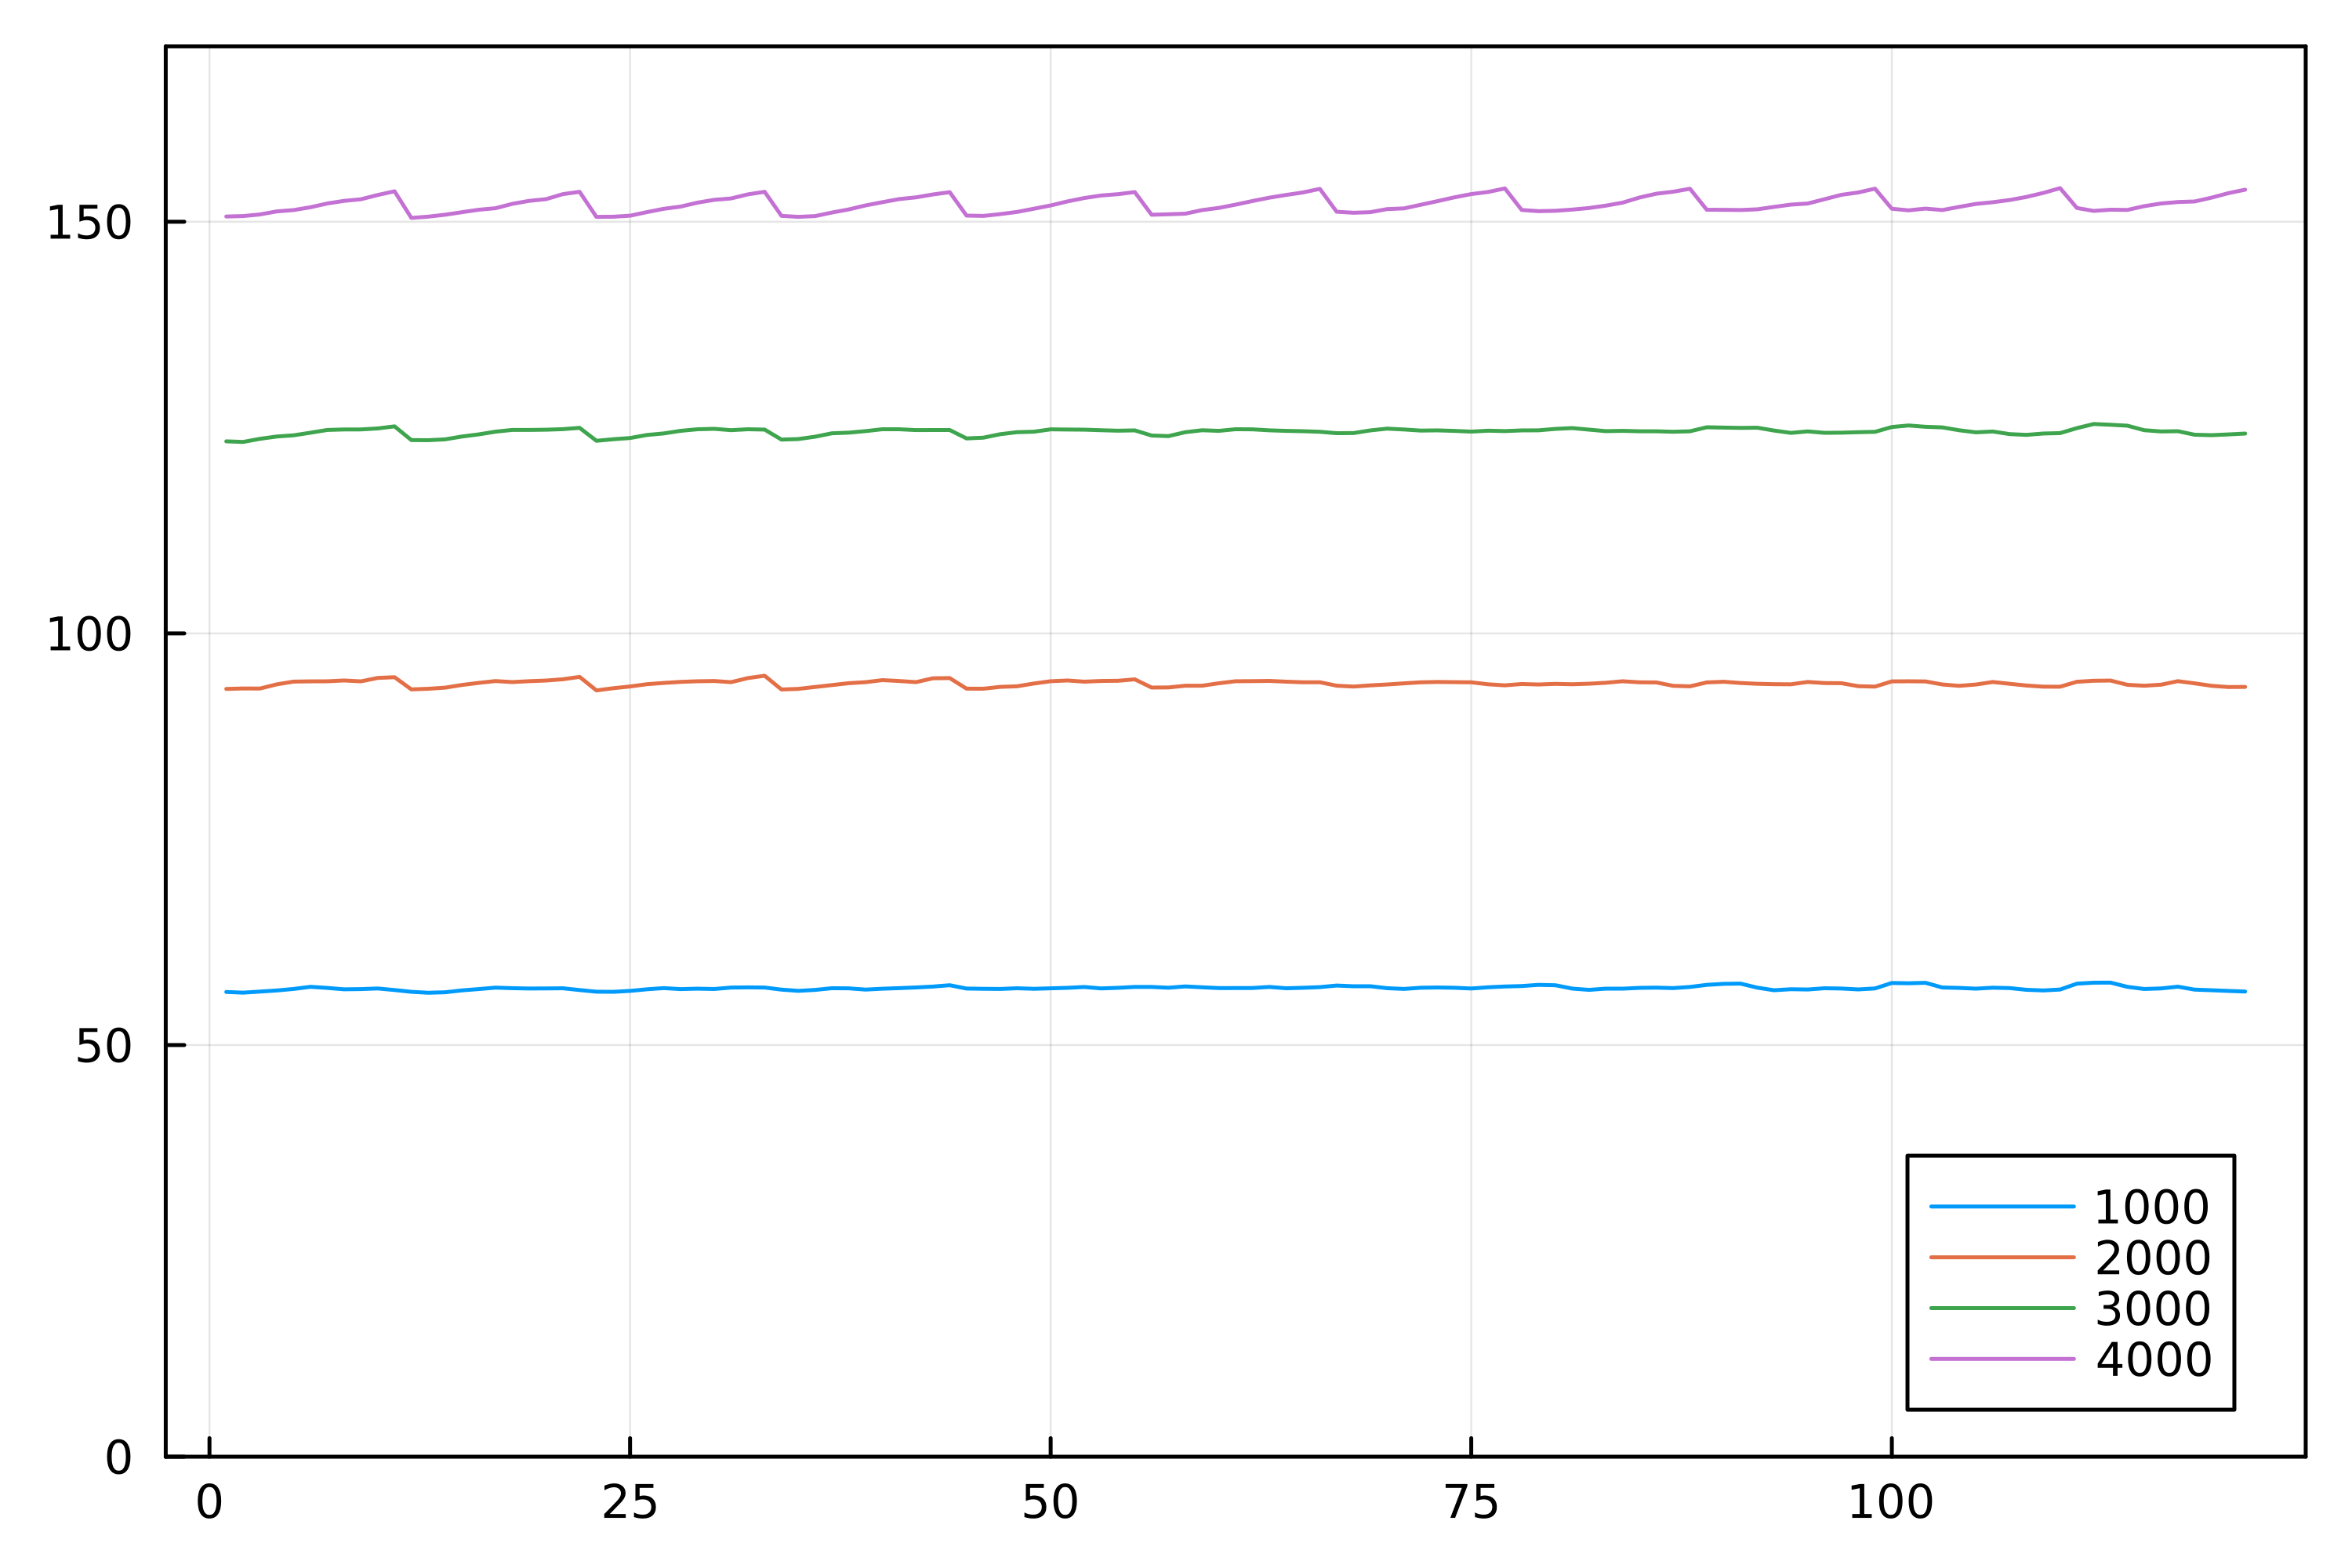
\includegraphics[width=\textwidth]{../data/energy/energies-different-blocks.png}
        \only<1>{    
        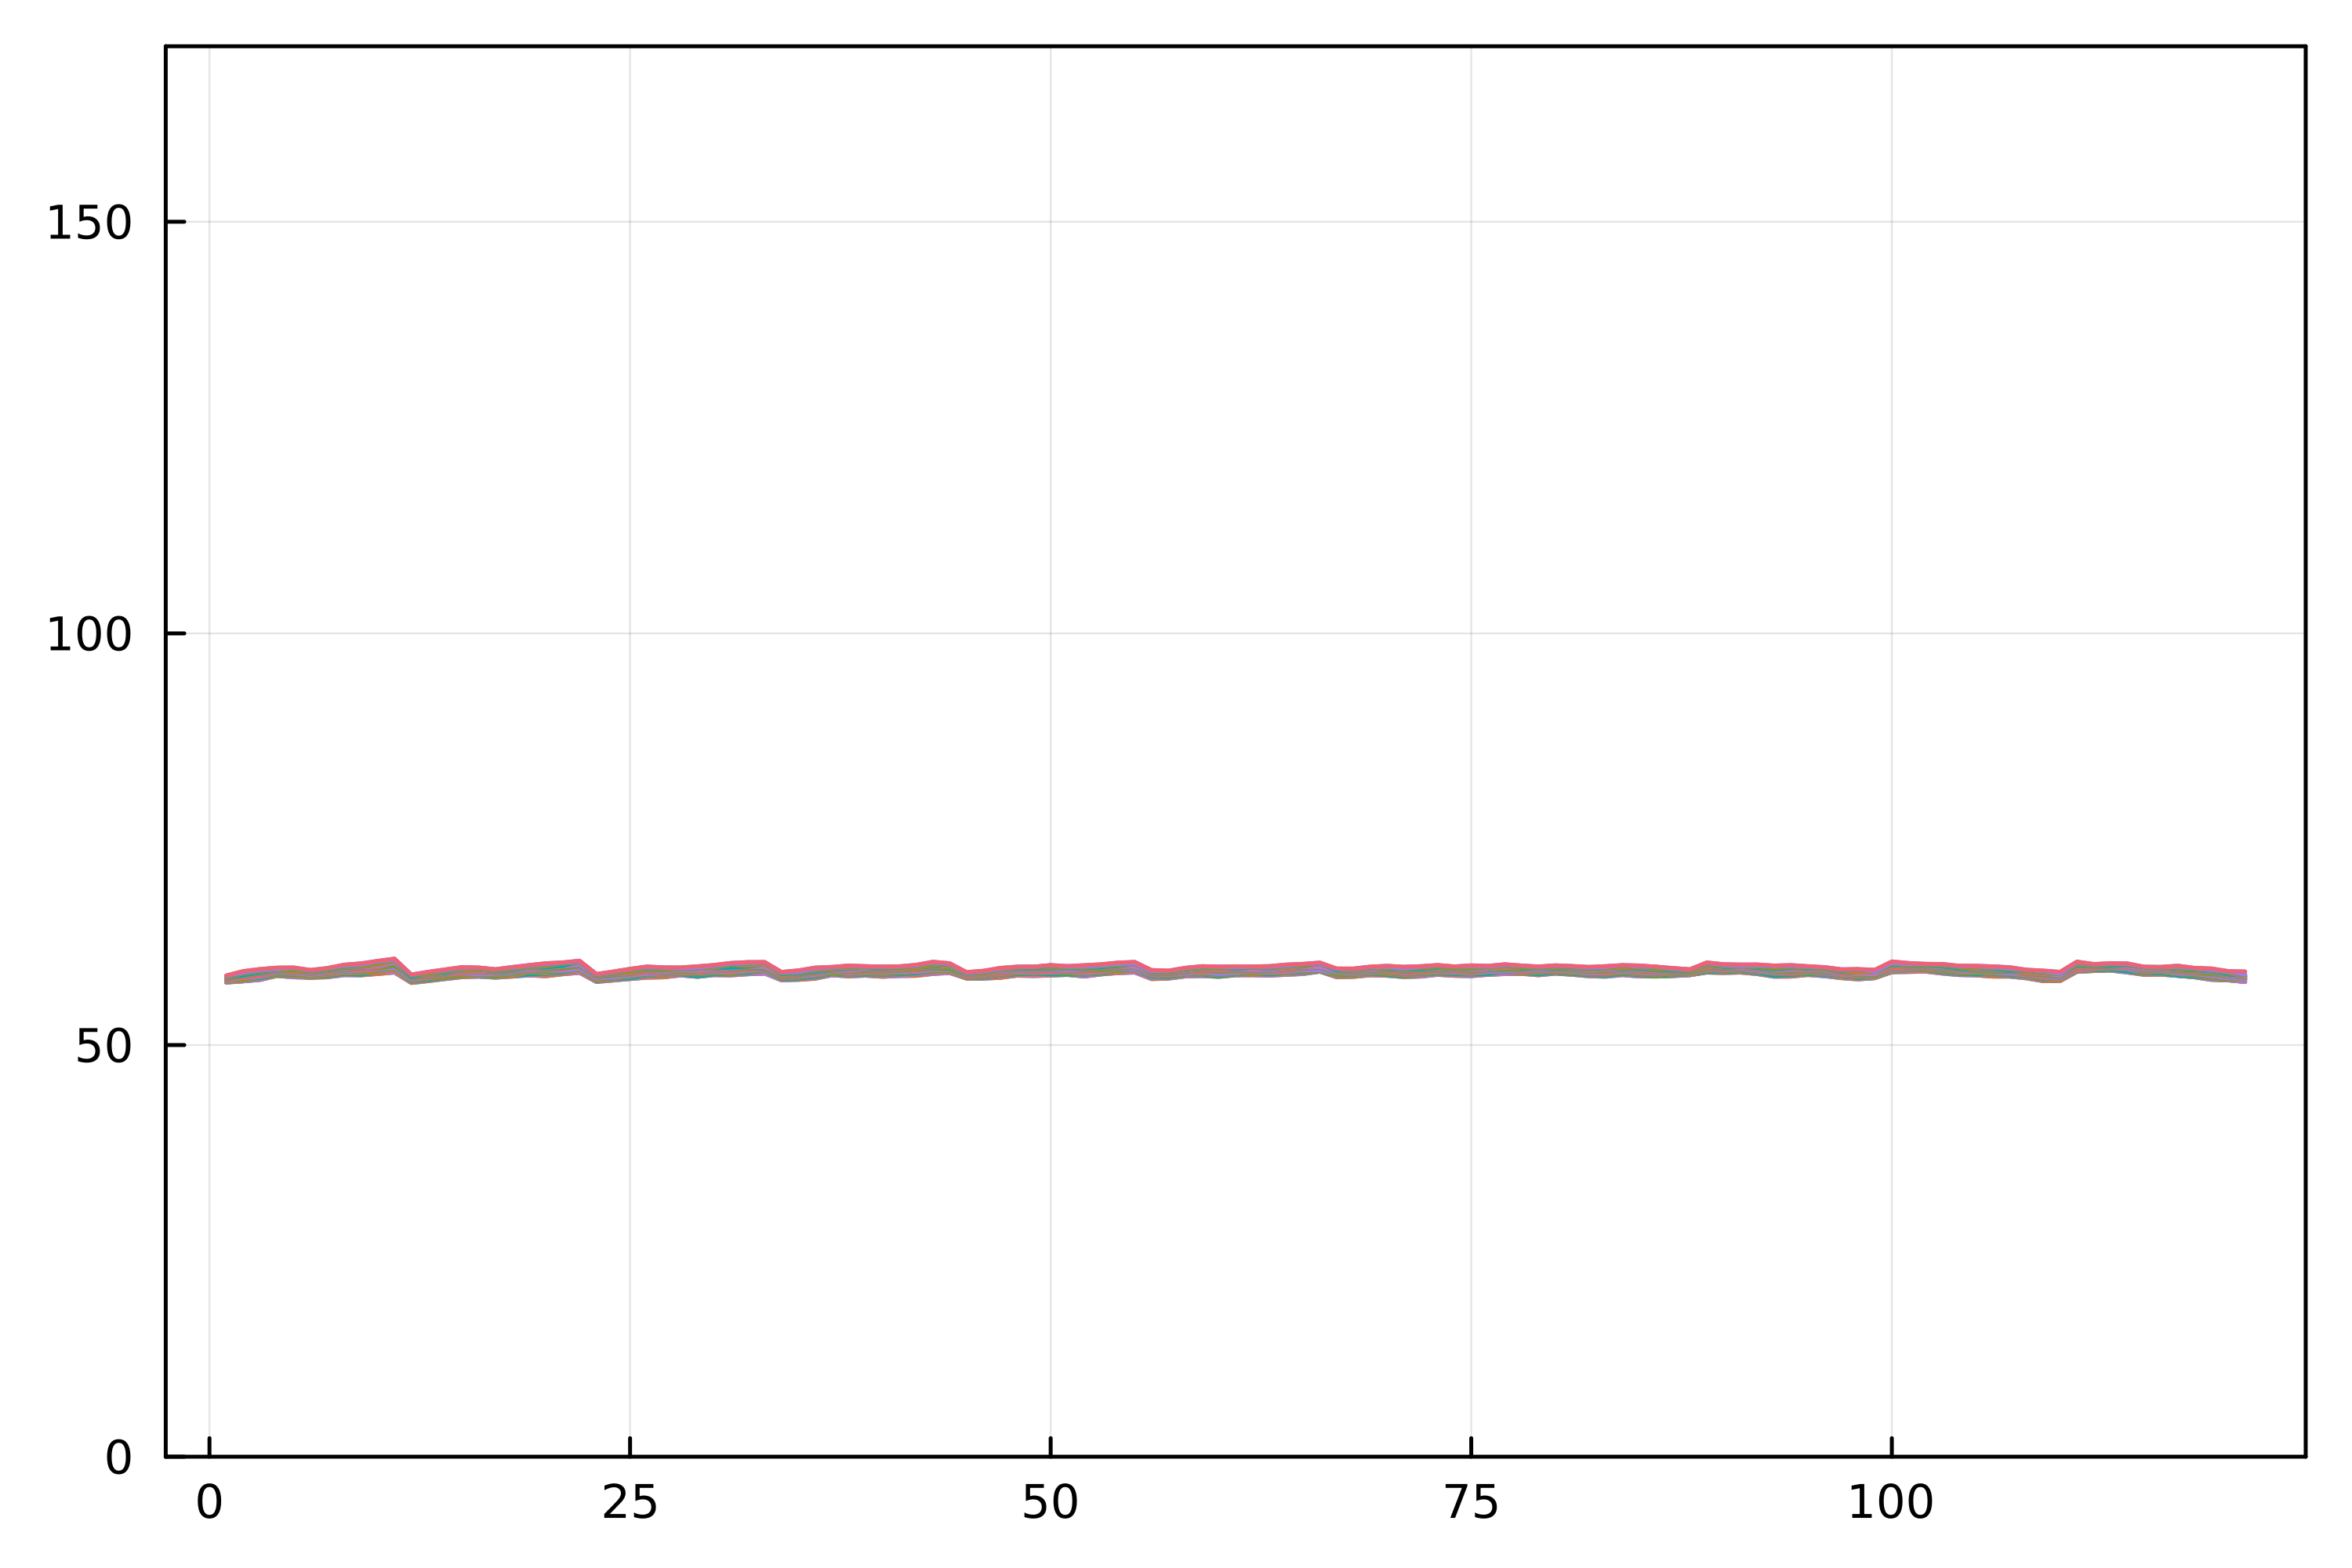
\includegraphics[width=\textwidth]{../data/energy/energies-same-blocks-1062.png}
        }
        \only<2>{
            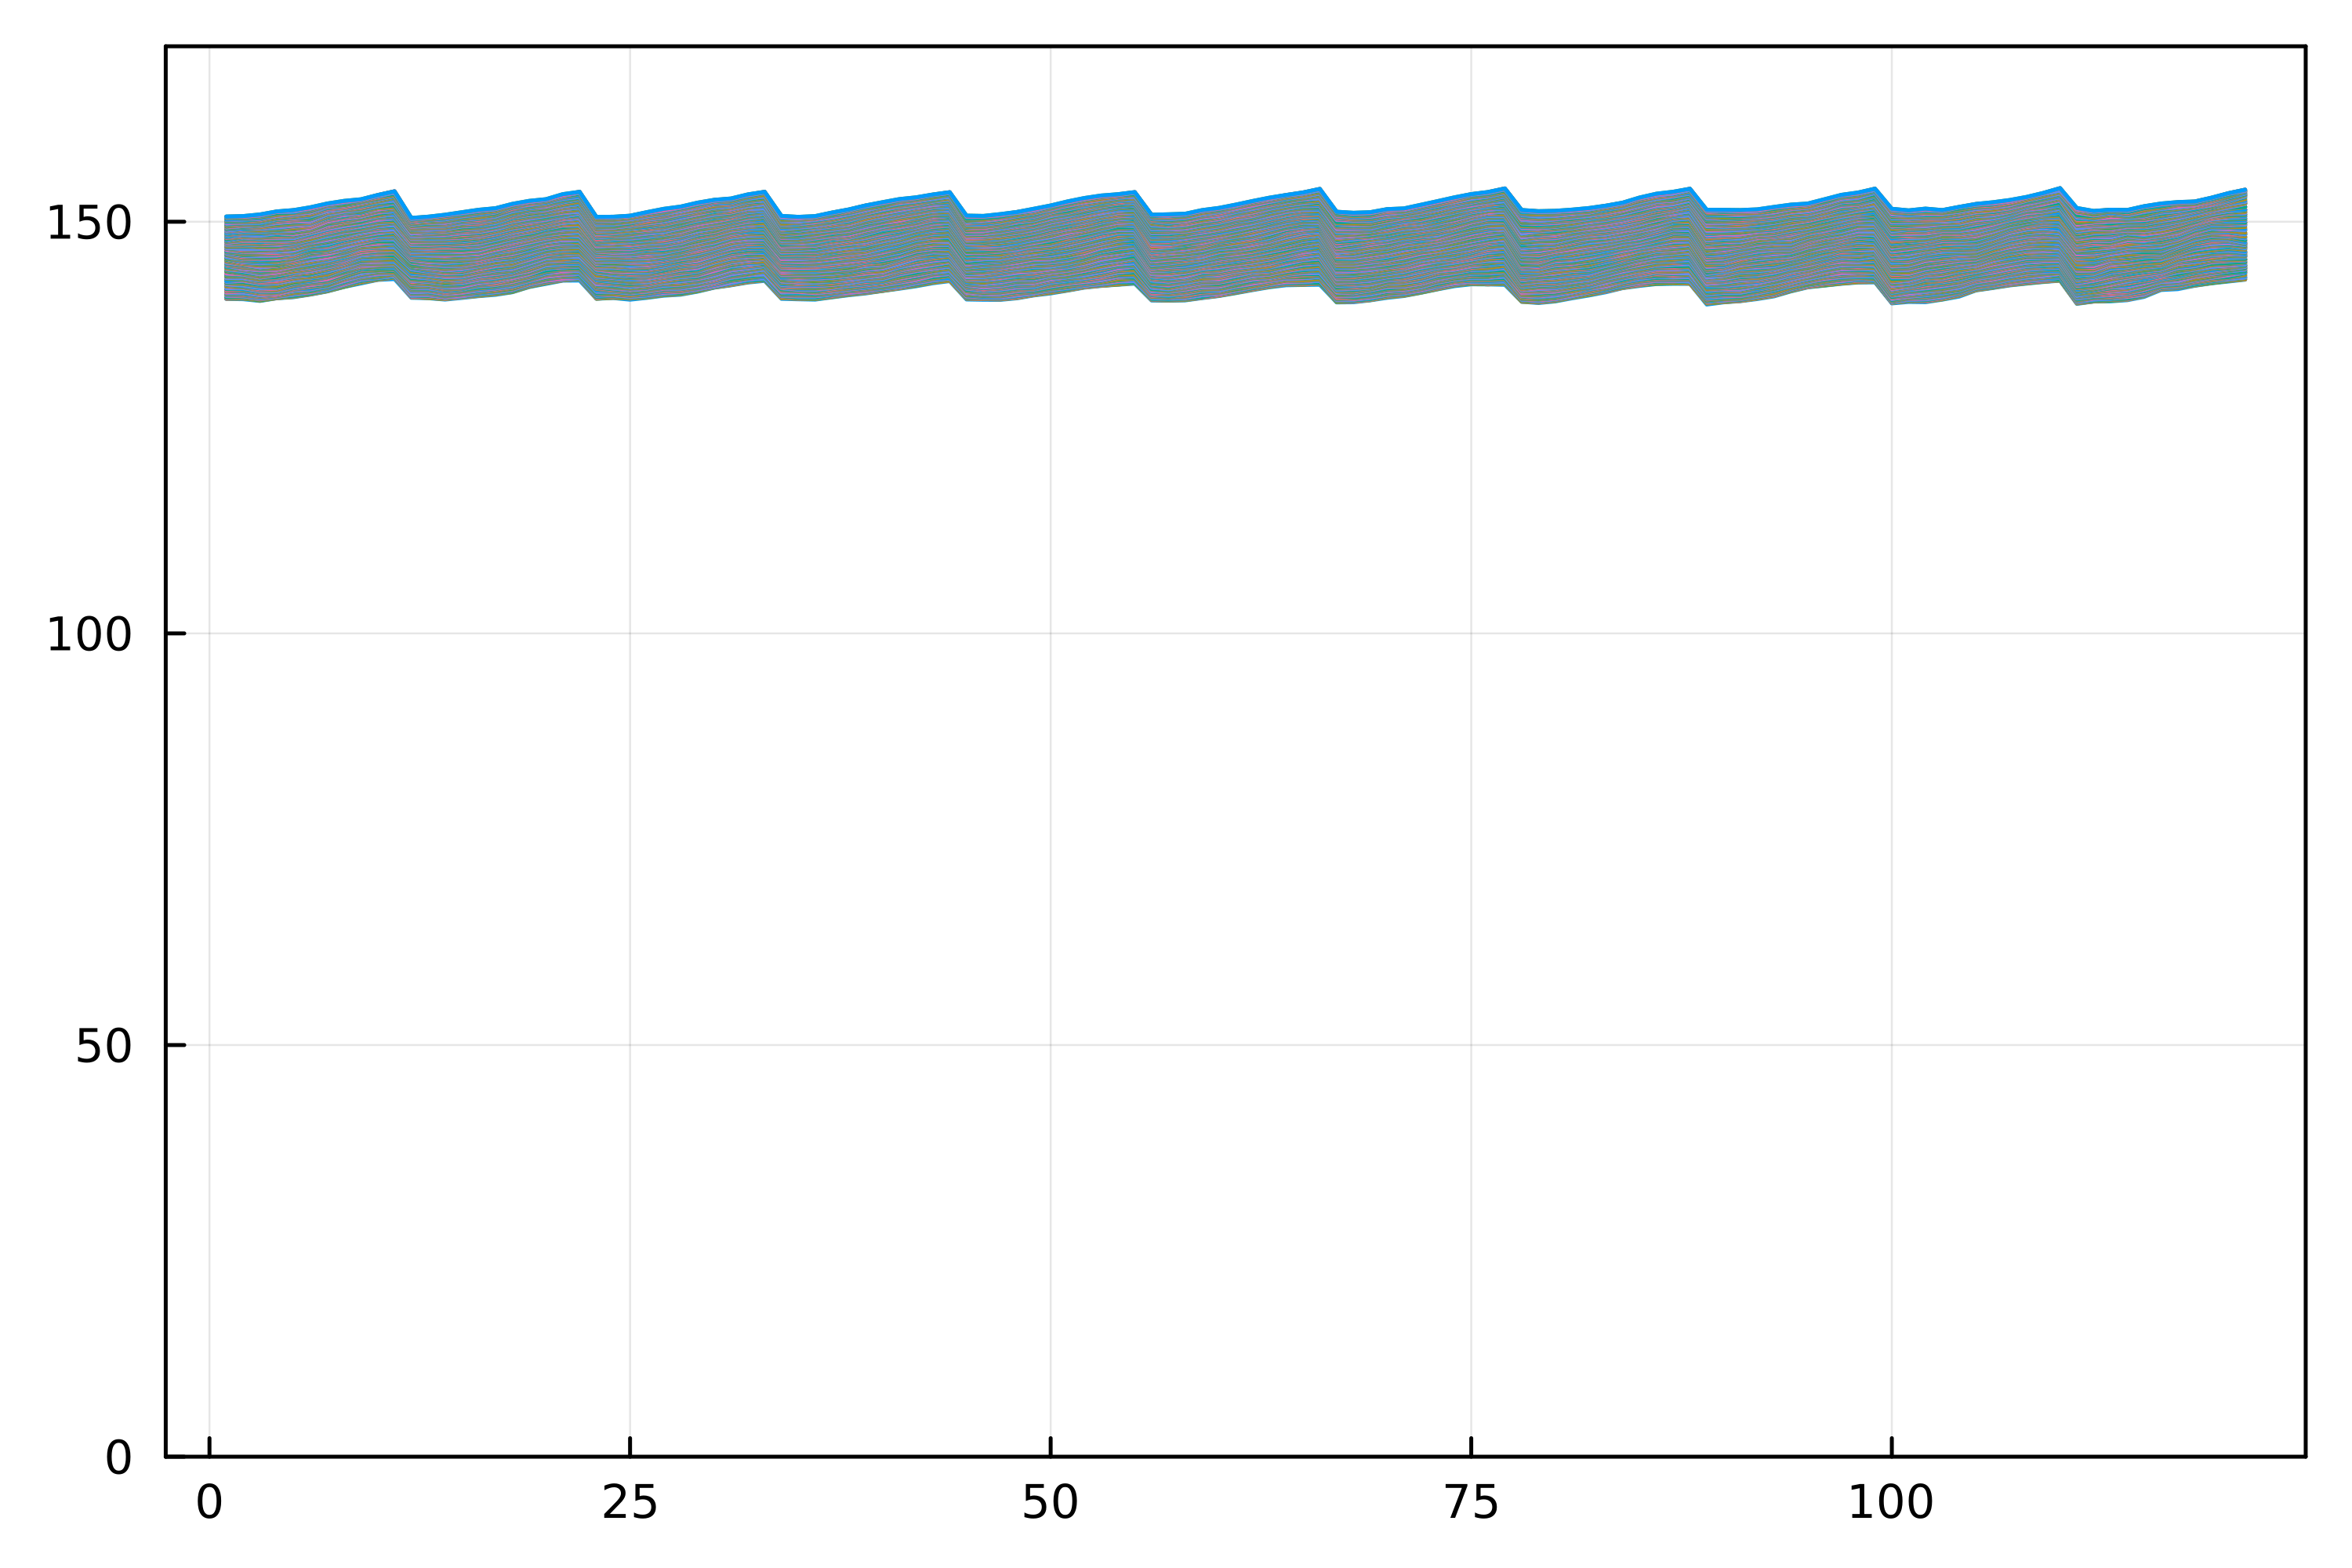
\includegraphics[width=\textwidth]{../data/energy/energies-same-blocks-4000.png}
        }
    \end{center}    
\end{column}

\end{columns}

\only<3>{
    \vspace{0.5cm}
    
    Thus in both $\chi$ and $\Sigma^{\text{CH}}$: 
    \begin{equation*}
        \begin{aligned}
             \sum_{n''}^{\text{high emp.}} M_{n'' n}^* M_{n'' n'} \times f(E_{n'' \vb{k}}) 
            = \sum_{\text{block $n_{\text{b}}$}}^{\text{high emp.}} f(\bar{E}_{n_{\text{b}}}) \sum_{n''}^{\text{block $n_{\text{b}}$}}
            M_{n'' n}^* M_{n'' n'}.
        \end{aligned}
    \end{equation*}
}

\end{frame}


\begin{frame}
\frametitle{Understanding \shortcode{pseudobands}: wave function averaging?}

For \shortcode{pseudobands} to work, we need 
\begin{equation}
    \begin{aligned}
        \underbrace{
            \sum_{n'' \in \text{block $n_{\text{b}}$}} M_{n'' n}^* M_{n'' n'} 
        }_{\text{normal}}
        &\sim M_{\text{averaged band}, n}^* M_{\text{averaged band}, n'} \\
        &= \underbrace{
            \sum_{n''_1, n''_2 \in \text{block $n_{\text{b}}$}} M_{n_1'' n'} M_{n_2'' n}^*
        }_{\text{pseudobands}}.
    \end{aligned}
    \label{eq:pseudobands-correct}
\end{equation}

\textbf{The question: is $[M_{n_1'' n'} M_{n_2'' n}^*]_{n_1'' n_2''}$ diagonal?}
Easy to verify: it's not.

\vspace{0.5cm}

\textbf{Then in which case is \eqref{eq:pseudobands-correct} correct in some sense?} 

\end{frame}

\section{Technical issues in calculating $M_{nn'}(\vb{k}, \vb{q}, \vb{G})$}

\begin{frame}
\frametitle{The structure of $\phi_{n \vb{k}}$}

\textbf{Plane wave basis} In BerkeleyGW \shortcode{WFN.h5}, 
\begin{equation*}
    \phi_{n \vb{k}}(\vb{r}, \sigma) = \frac{1}{\sqrt{V}} \sum_{\vb{G}} \ee^{\ii (\vb{k} + \vb{G}) \cdot \vb{r}} c_{n \vb{k}, \vb{G} \sigma}.
\end{equation*}    
Thus 
\begin{equation*}
    M_{nn'}(\vb{k}, \vb{q}, \vb{G}) 
    = \mel*{n \vb{k} + \vb{q}}{\ee^{\ii (\vb{q} + \vb{G}) \cdot \vb{r}}}{n' \vb{k}} 
    = \sum_{\vb{G}', \sigma} c^*_{n \vb{k} + \vb{q}, \vb{G} + \vb{G}' \sigma} c_{n \vb{k}, \vb{G}' \sigma}.
\end{equation*}

\textbf{Cutoff} Each $\vb{k}$ has its own $\vb{G}$-grid ($\sim 30000$ vectors for \SI{80}{Ry}).

\end{frame}

\begin{frame}
\frametitle{Procedure}

\textbf{Input} 
\begin{itemize}
    \item indices of $\vb{k}, \vb{q}$ in $\vb{k}$-grid; 
    \item index of $\vb{G}$ in $\vb{G}$-grid of $\vb{k}$ 
    (expect a $\vb{G}$ in $GW$ $\vb{G}$-grid, 
    cutoff = say \SI{30}{Ry}, not \SI{80}{Ry});
    \item $n, n'$.
\end{itemize}

\textbf{Procedure}
\begin{enumerate}
    \item find index of $\vb{k}$
    \item find index of $\vb{G} + \vb{G}'$ in $\vb{G}$-grid of $\vb{k} + \vb{q}$,
    for each $\vb{G}'$ in $\vb{G}$-grid of $\vb{k}$
    \item do summation $\sum_{\vb{G}', \sigma} c^*_{n \vb{k} + \vb{q}, \vb{G} + \vb{G}' \sigma} c_{n \vb{k}, \vb{G}' \sigma}$.
\end{enumerate}    

\vspace{0.3cm}

\textbf{Performance} Main bottleneck: finding $\vb{G} + \vb{G}'$.
Using \shortcode{StaticArrays.jl} helps a lot! 

\end{frame}

\section{\shortcode{pseudobands} for $\chi$}

\begin{frame}
\frametitle{$\chi$ revisited}

\begin{columns}

\begin{column}{0.5\textwidth}
    Under GPP:
    \small
    \begin{equation*}
    \begin{aligned}
        &\quad \chi_{\vb{G} \vb{G}'}(\vb{q}, \omega=0)^{\text{pseudobands}} \\
        &\approx \sum_{\vb{k}} \sum_{\text{block $n_{\text{b}}$}}^{\text{emp}} 
        \frac{
            2
        }{
            E_{n, \vb{k} + \vb{q}} - E_{\text{average in block $n_{\text{b}}$}} 
        } \\
        &\quad \times \sum_{n'_{1,2} \in \text{block $n_{\text{b}}$}} \sum_{n}^{\text{occ}} 
        M_{n n'_1} (\vb{k}, \vb{q}, \vb{G}) M^*_{nn'_2} (\vb{k}, \vb{q}, \vb{G}') 
    \end{aligned}
    \end{equation*}
    \normalsize

    \only<1>{
        \textbf{Our goal} Show that  
        \begin{equation*}
            \sum_{n}^{\text{occ}} 
                M_{n n'_1} (\vb{k}, \vb{q}, \vb{G}) M^*_{nn'_2} (\vb{k}, \vb{q}, \vb{G}') 
        \end{equation*}
        is diagonal for \shortcode{pseudobands} to work.
    }

    \only<2-4>{
        For $\vb{G} = \vb{G}'$, $\sum_{n}\limits^{\text{occ}} 
        M_{n n'_1} (\vb{k}, \vb{q}, \vb{G}) M^*_{nn'_2} (\vb{k}, \vb{q}, \vb{G}') $
        is diagonal.
    }

    \only<4>{
        Strikingly, $\scriptstyle \sum_{n}^{\text{occ}} M_{n n'_1} (\vb{k}, \vb{q}, \vb{G}) M^*_{nn'_2} (\vb{k}, \vb{q}, \vb{G}')$ is still very diagonal for bands near Fermi surface!
    }

    \only<5>{
        When $\vb{G} \neq \vb{G}'$, $\sum_{n}\limits^{\text{occ}} 
        M_{n n'_1} (\vb{k}, \vb{q}, \vb{G}) M^*_{nn'_2} (\vb{k}, \vb{q}, \vb{G}') $
        is not diagonal at all.
    }
    
    \only<6>{
        But since $E_{n \vb{k} + \vb{q}} \ll E_{\text{average in block $n_{\text{b}}$}}$, the $1 / \Delta E$ factor is a constant w.r.t. $\vb{k}$, 
        and after summing over $\vb{k}$, $MM^*$ becomes diagonal.
    }
\end{column}

\begin{column}{0.5\textwidth}
    
\only<2>{
    \begin{center}
        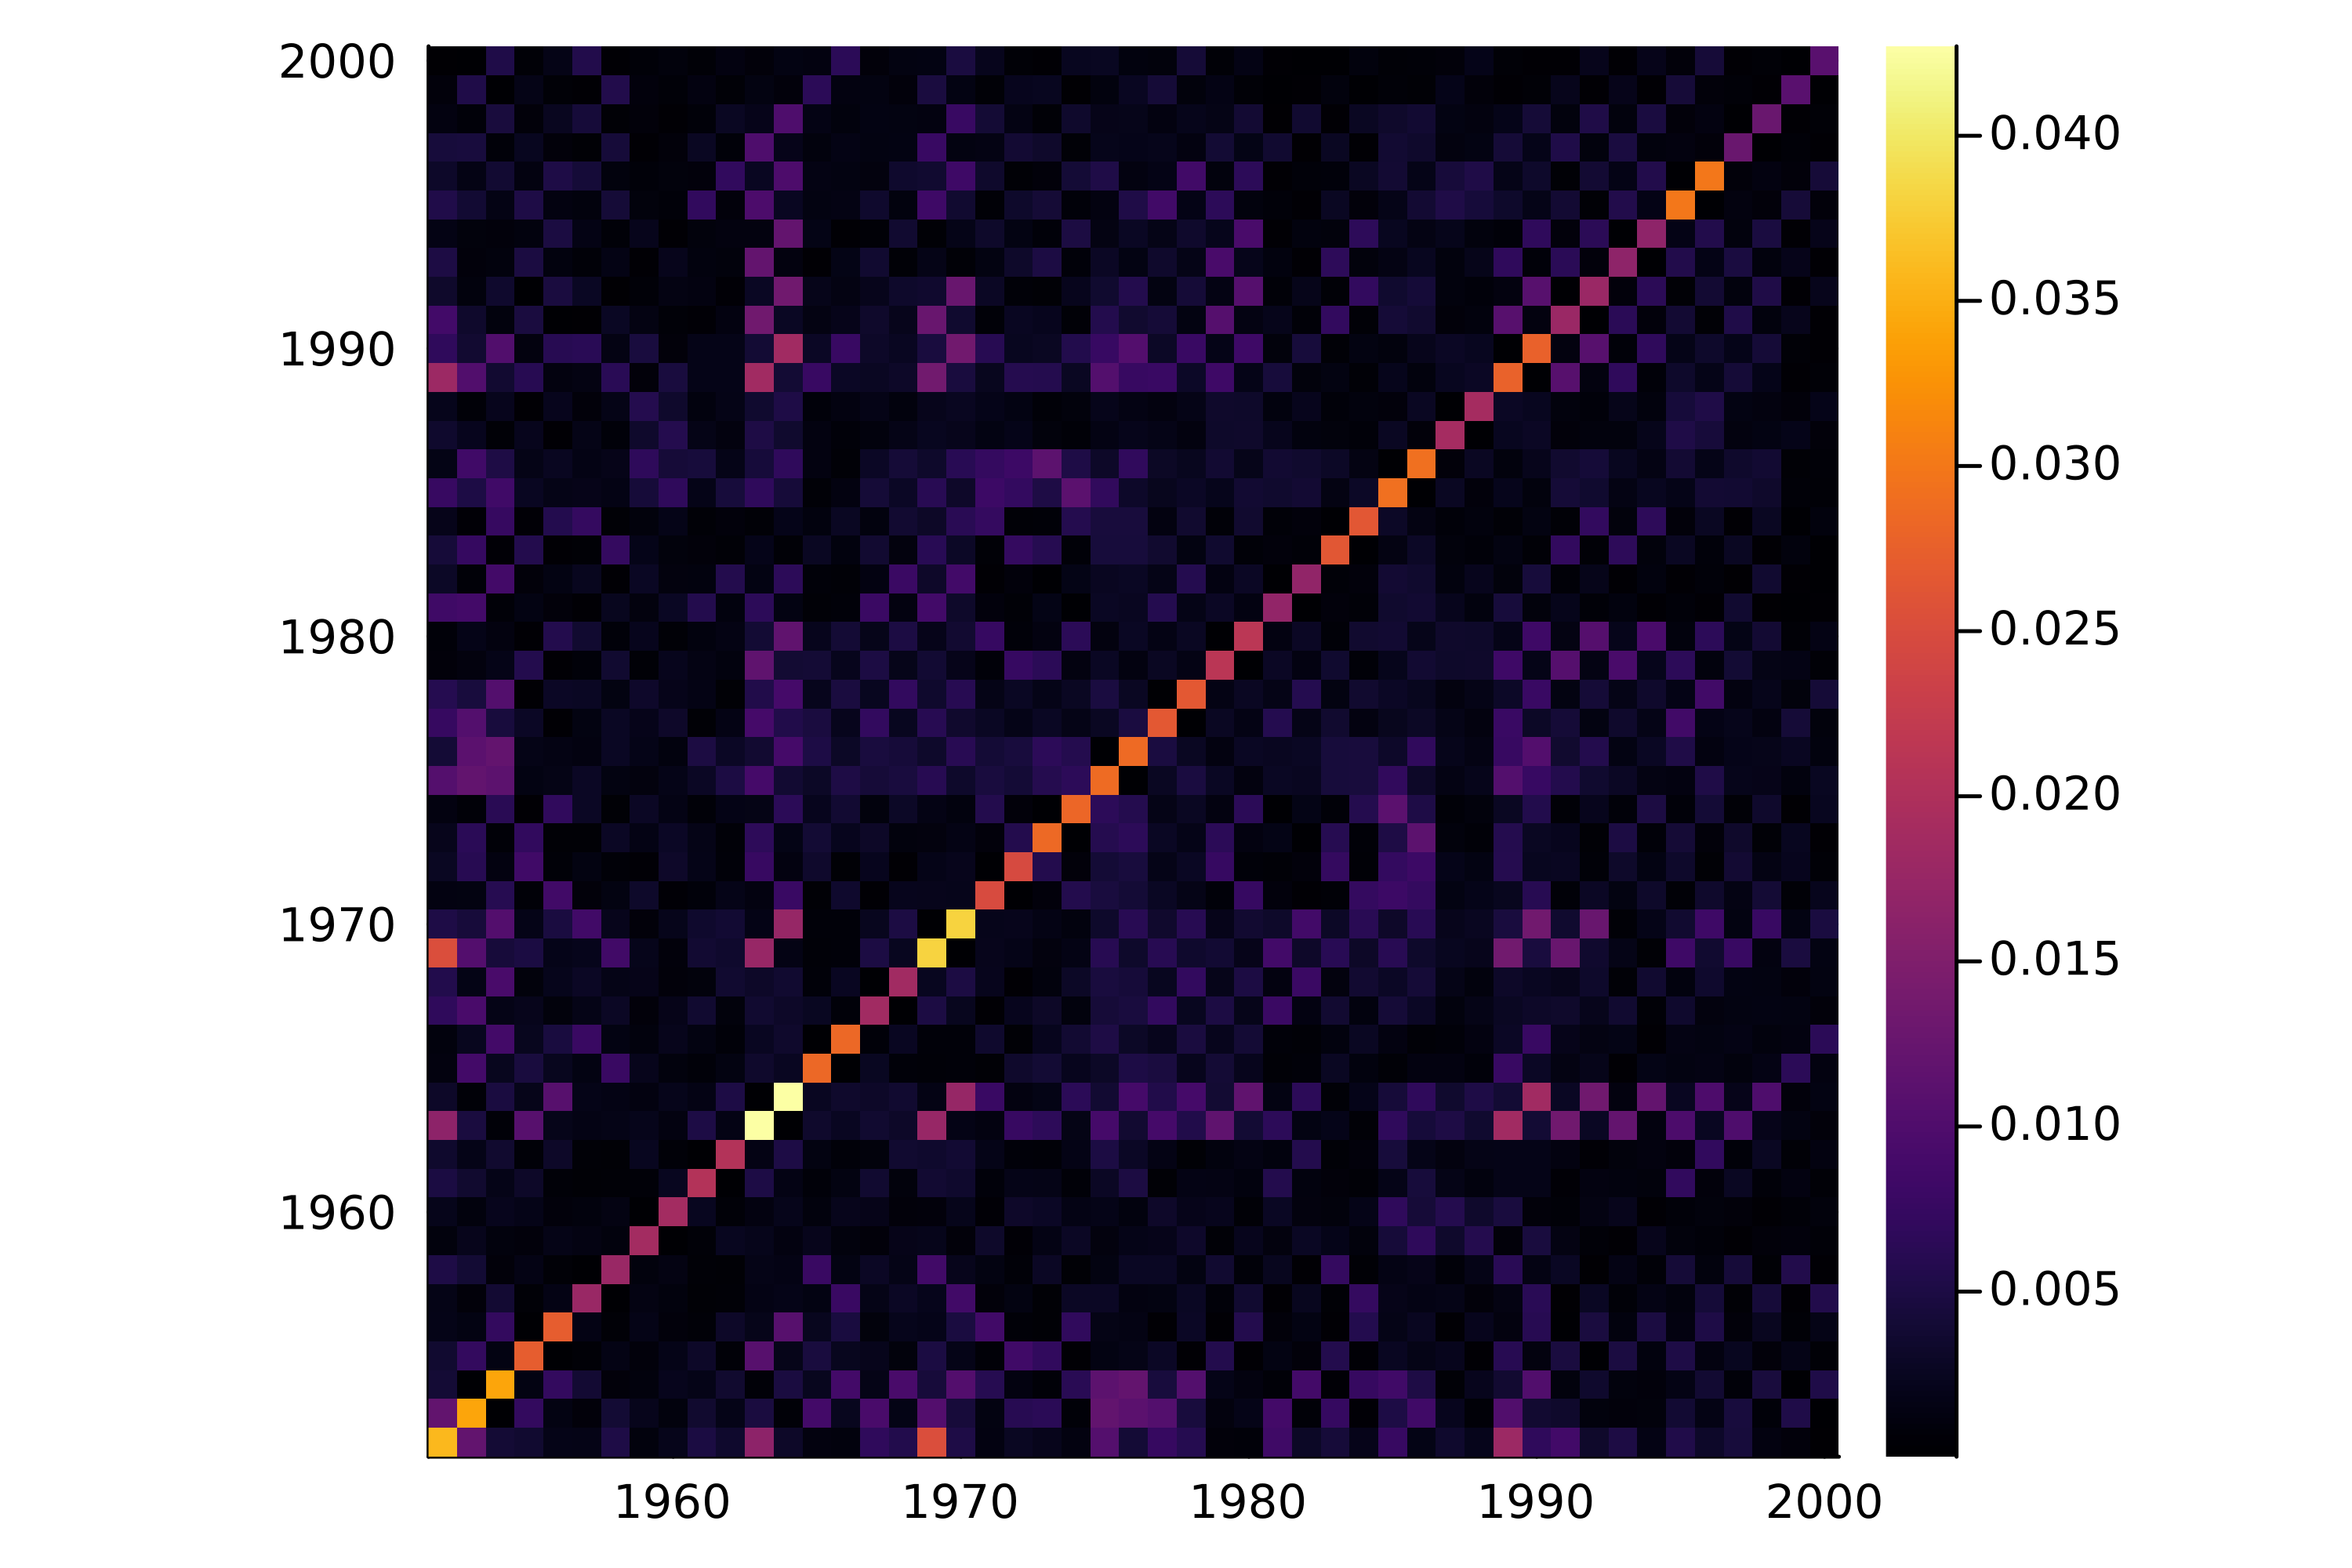
\includegraphics[width=\textwidth]{../data/chi/nc_range-1951-2000-k_idx-1-q_idx-1-G_idx-810.png}
    \end{center}

    \small
    The same \ce{WTe2} run, $\vb{G} = (0, 1, -14), \vb{k} = \vb{k}_2 = (0, 0.00, 0), \vb{q} = (0, 0.00, 0)$
    \normalsize
}

\only<3>{
    \begin{center}
        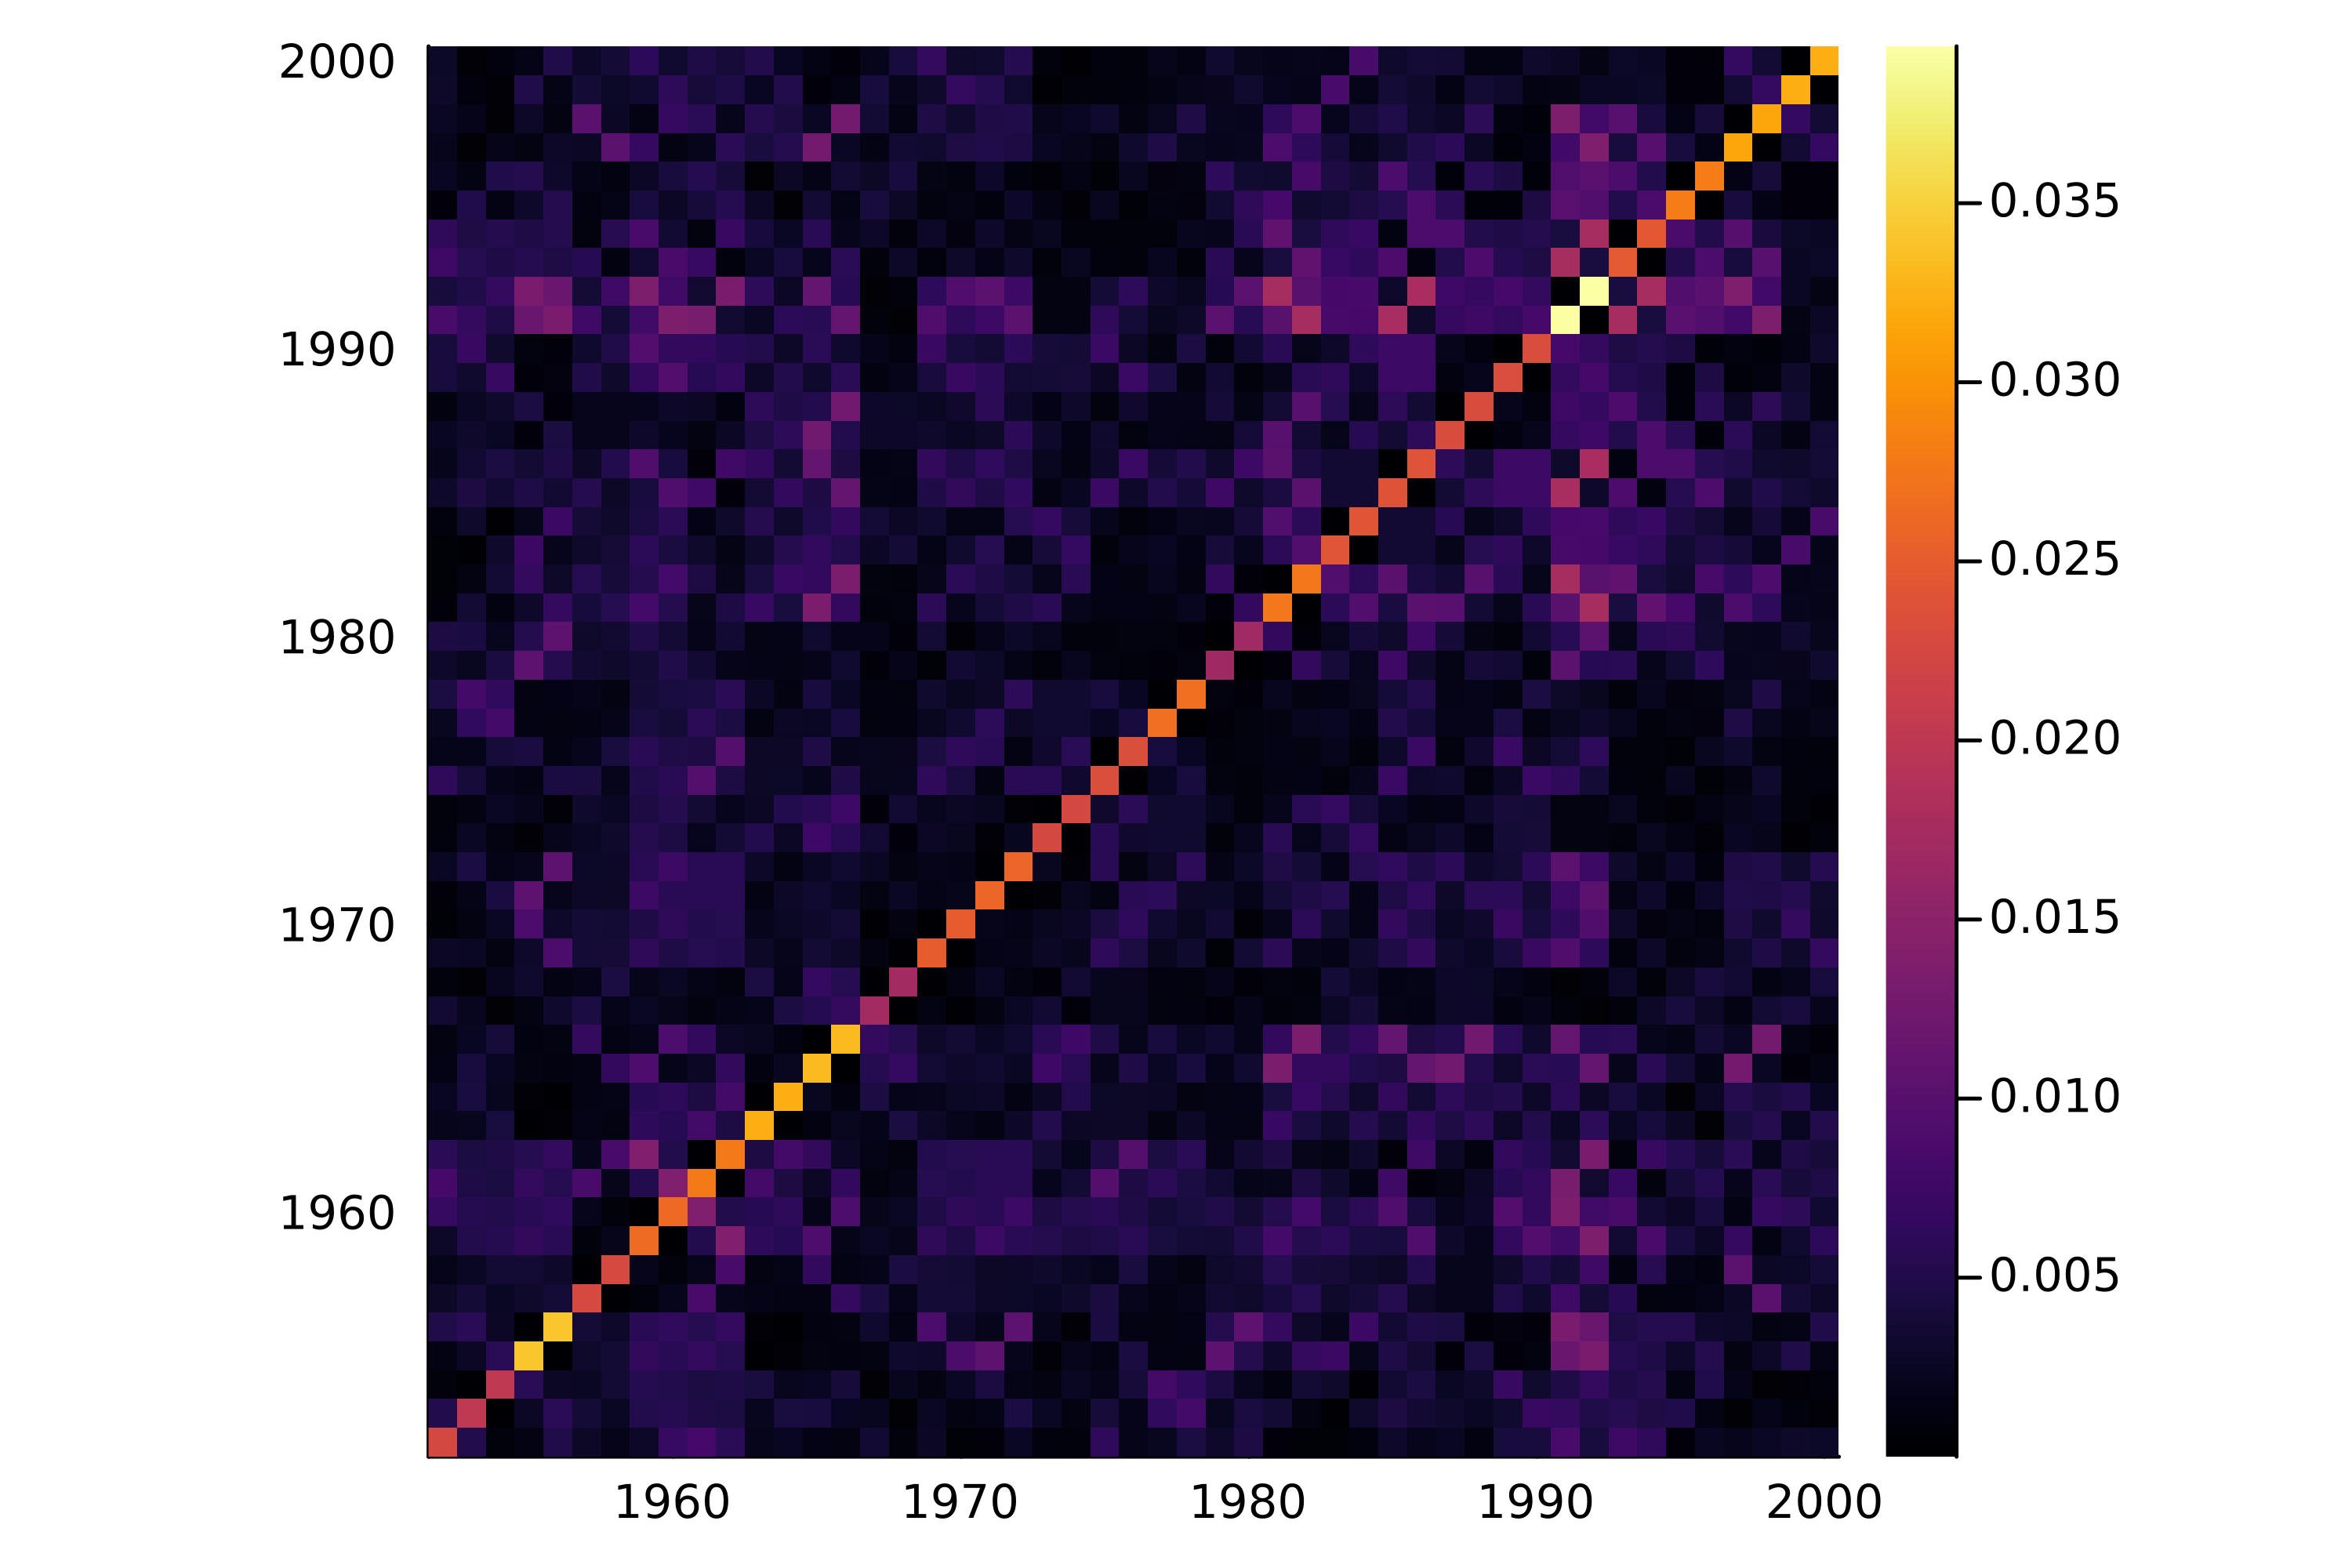
\includegraphics[width=\textwidth]{../data/chi/nc_range-1951-2000-k_idx-2-q_idx-3-G_idx-810.png}
    \end{center}
    
    \small
    The same \ce{WTe2} run, $\vb{G} = (0, 1, -14), \vb{k} = \vb{k}_2 = (0, 0.05, 0), \vb{q} = (0, 0.10, 0)$
    \normalsize
}

\only<4>{
    \begin{center}
        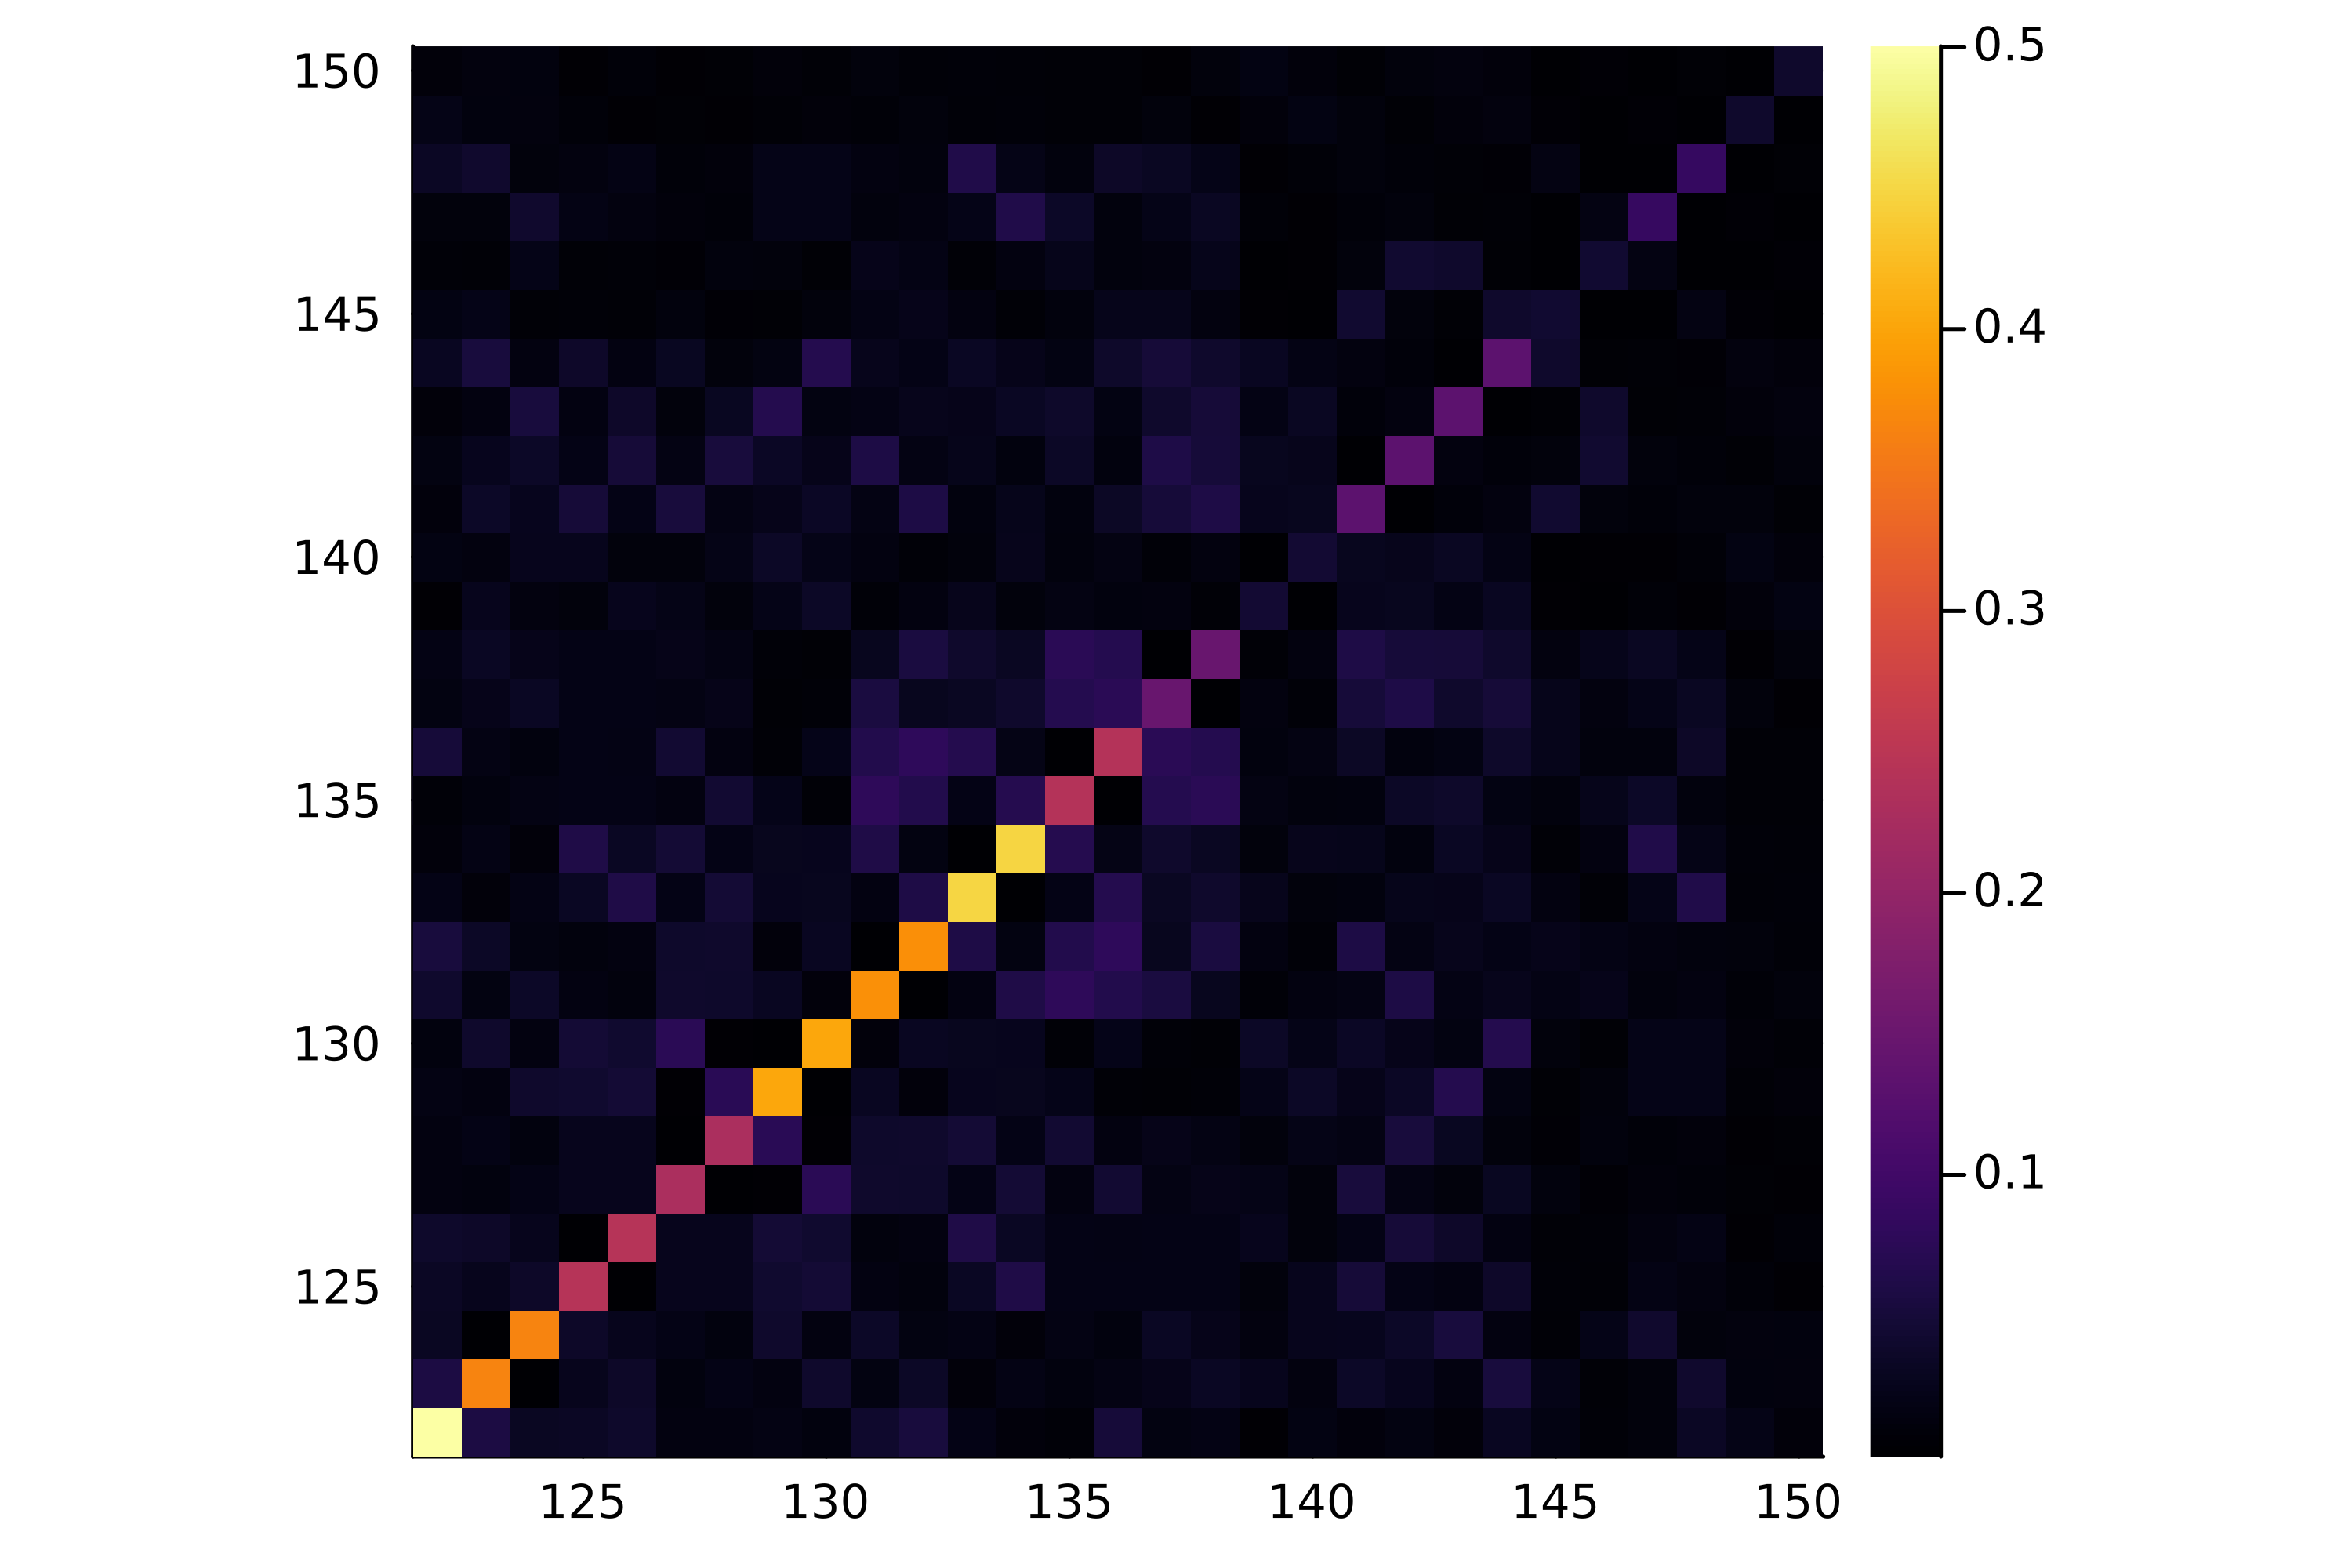
\includegraphics[width=\textwidth]{../data/chi/nc_range-121-150-k_idx-2-q_idx-3-G_idx-100.png}
    \end{center}

}

\only<5>{
    \begin{center}
        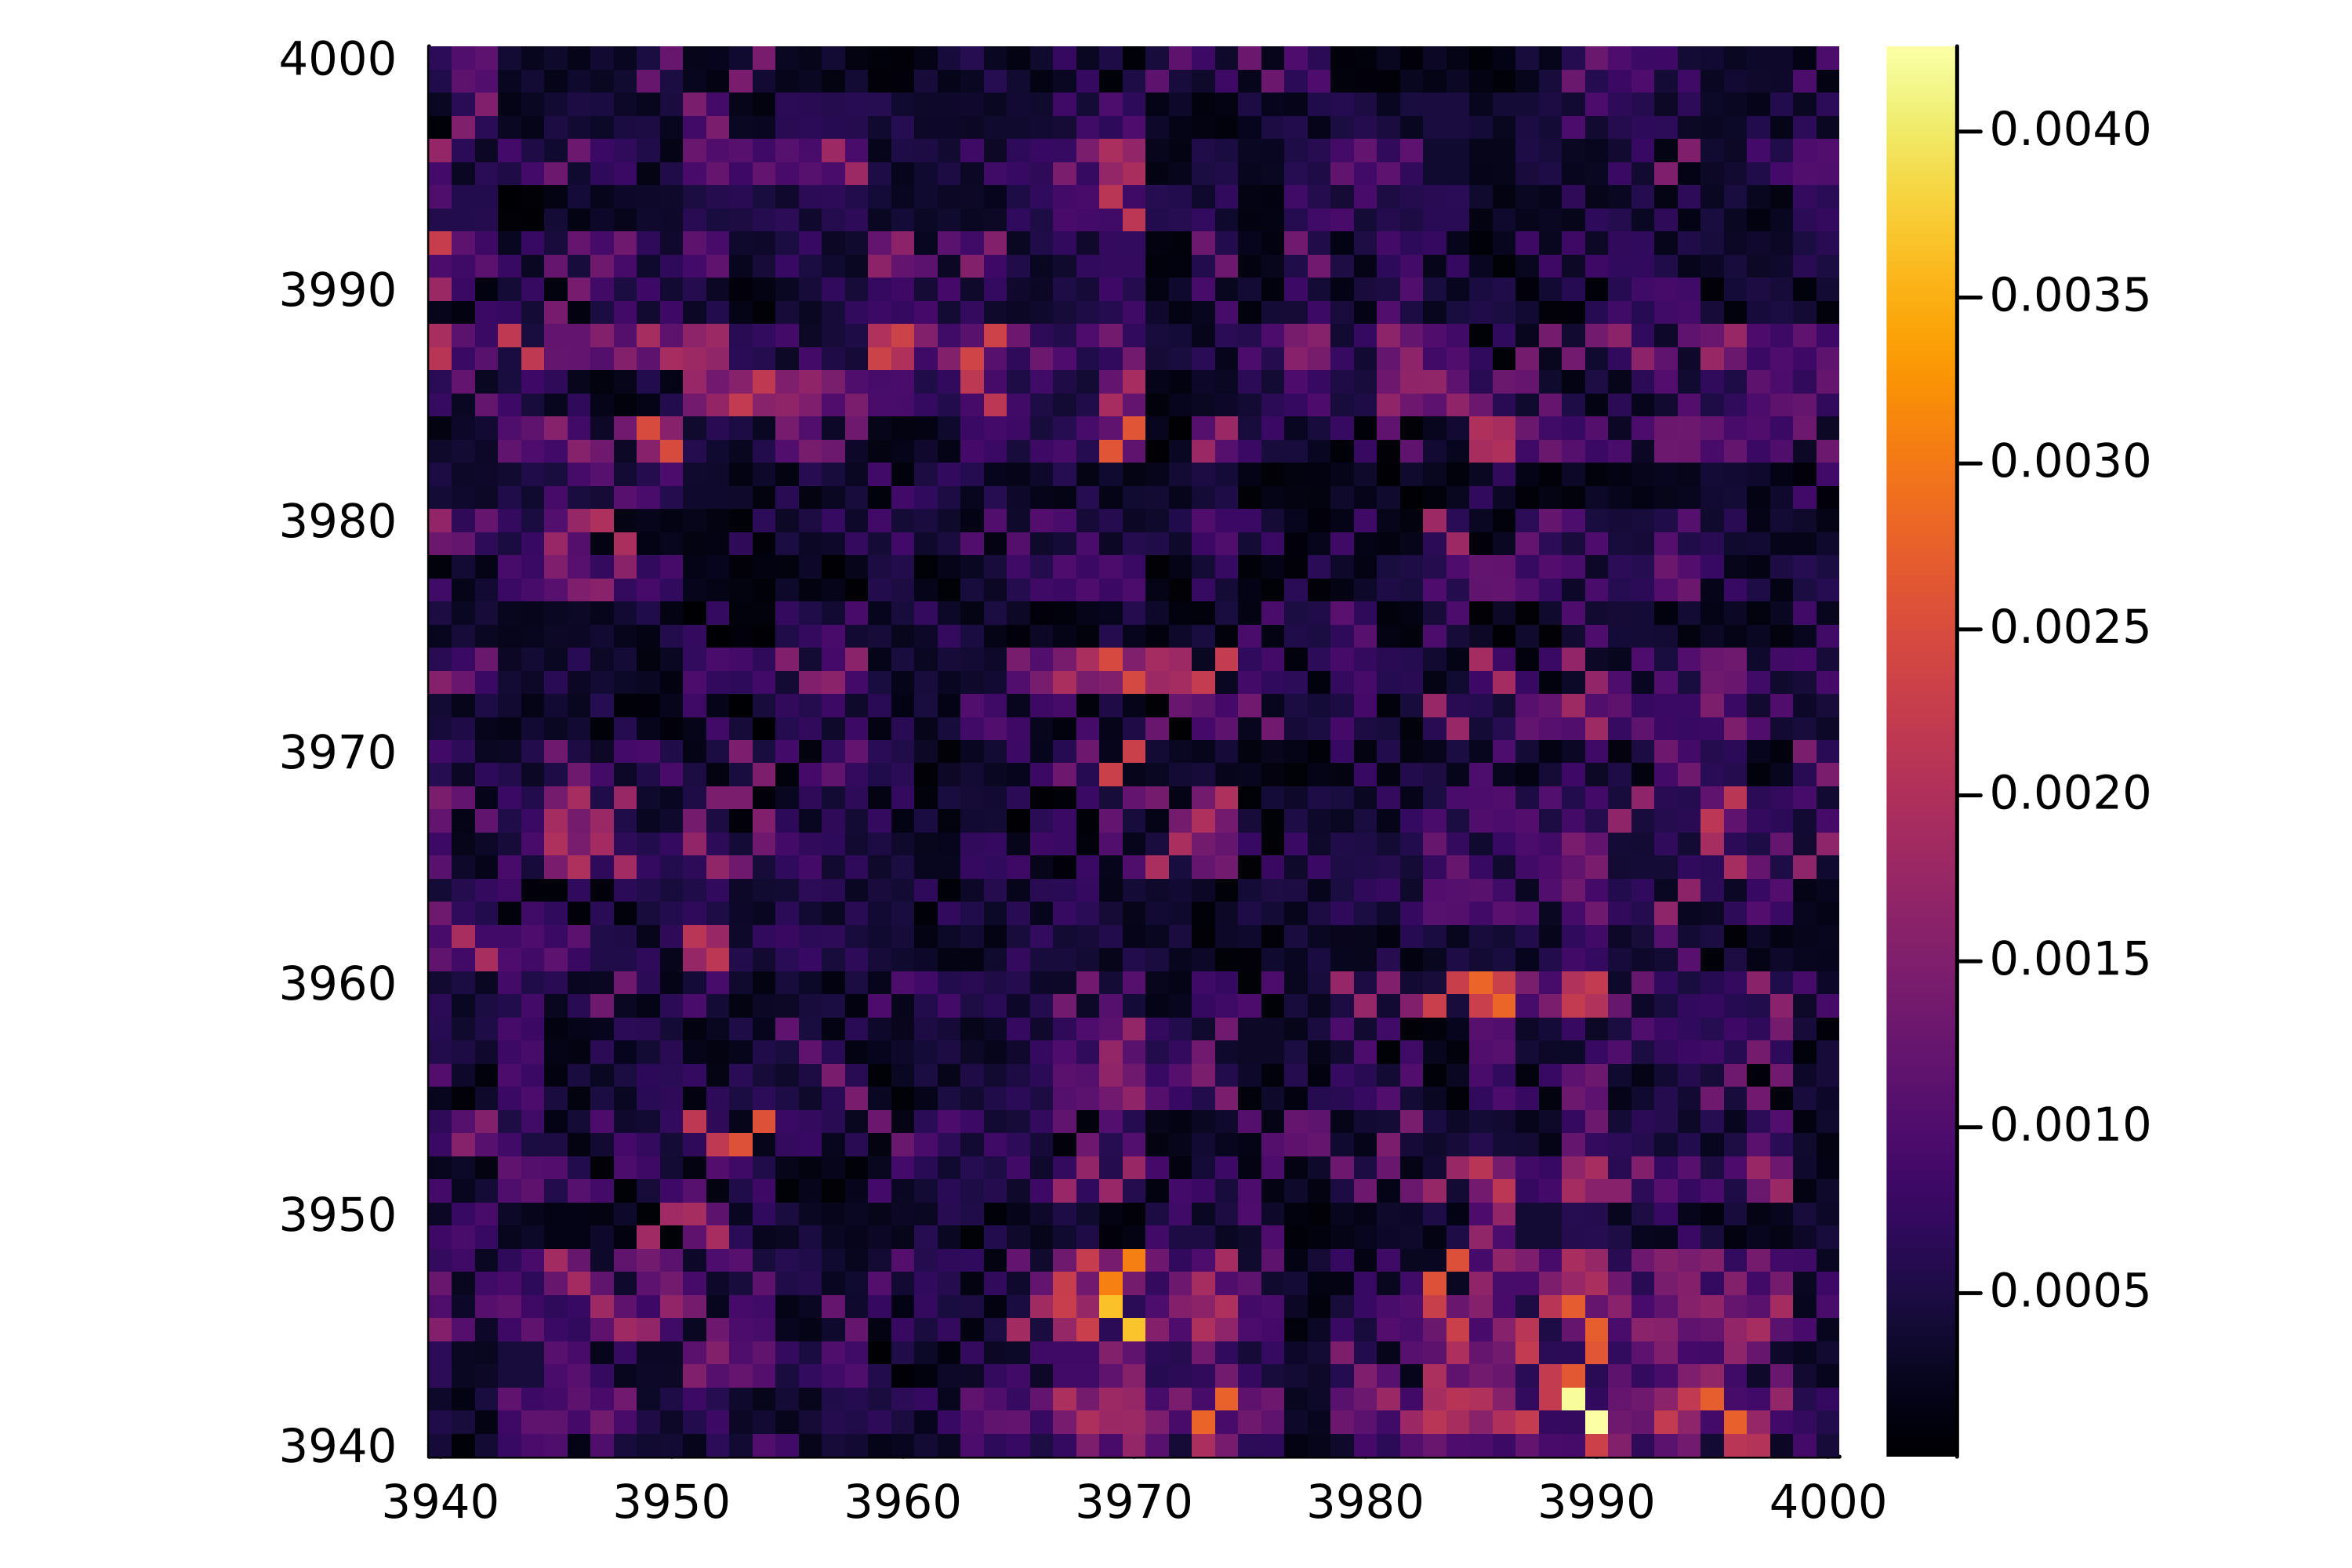
\includegraphics[width=\textwidth]{../data/chi/nc_range-3939-4000-k_idx-2-q_idx-3-G1_idx-2000-G2_idx-2001.png}
    \end{center}
    
}

\only<6>{
    \begin{center}
        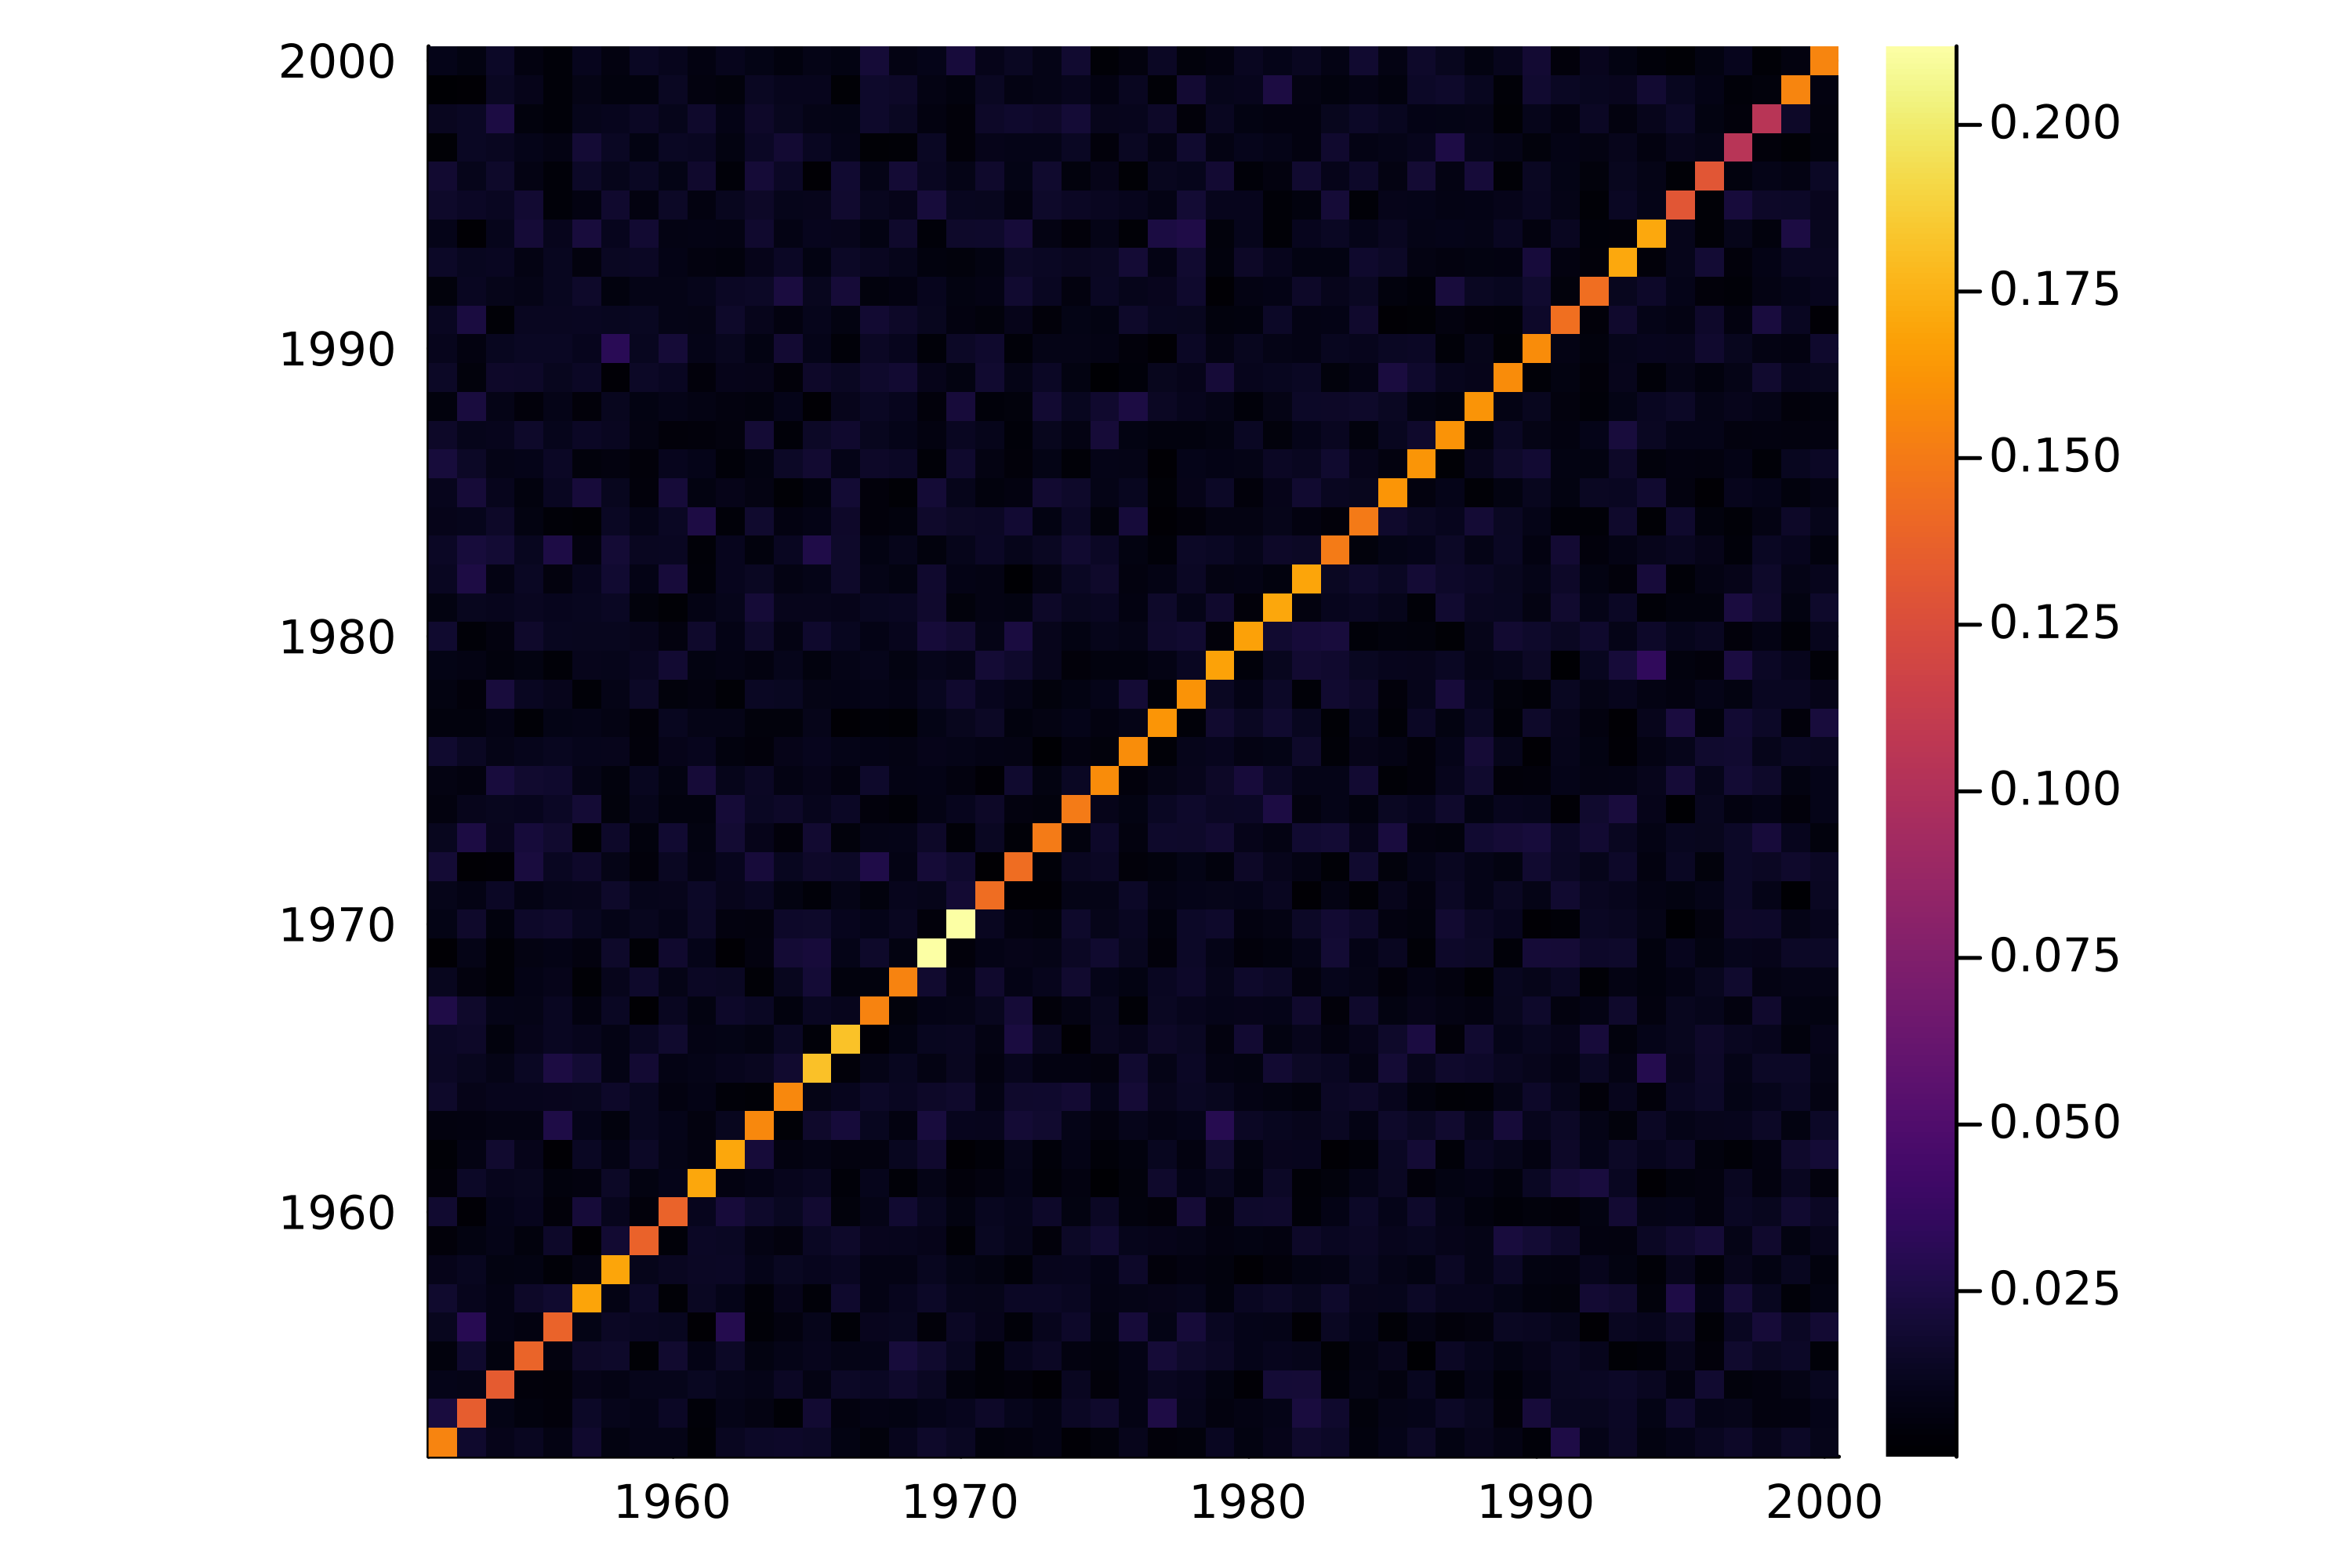
\includegraphics[width=\textwidth]{../data/chi/nc_range-1951-2000-k_sum-q_idx-9-G1_idx-200-G2_idx-204.png}
    \end{center}
}


\end{column}

\end{columns}

\end{frame}


\begin{frame}
\frametitle{Half-way generalization about \shortcode{pseudobands} in $\chi$}

\begin{itemize}
    \item[\faHandPointRight] \shortcode{pseudobands} works  
    when it's necessary to do so 
    \item[\faHandPointRight] What prevents \shortcode{pseudobands} from working 
    around Fermi surface is the energy dispersion
\end{itemize}

\vspace{0.5cm}

\dots but do we have any theoretical explanation for this?

\end{frame}

\begin{frame}
\frametitle{Cancellation of cross-terms in $\chi$}

\begin{columns}
    
\begin{column}{0.6\textwidth}
    $y$ axis: $\scriptstyle M_{n n'_1} (\vb{k}, \vb{q}, \vb{G}) M^*_{nn'_2} (\vb{k}, \vb{q}, \vb{G}')$, $n_1' \neq n_2'$
    $x$ axis: $n$ (occupied band index) 
    \begin{center}
        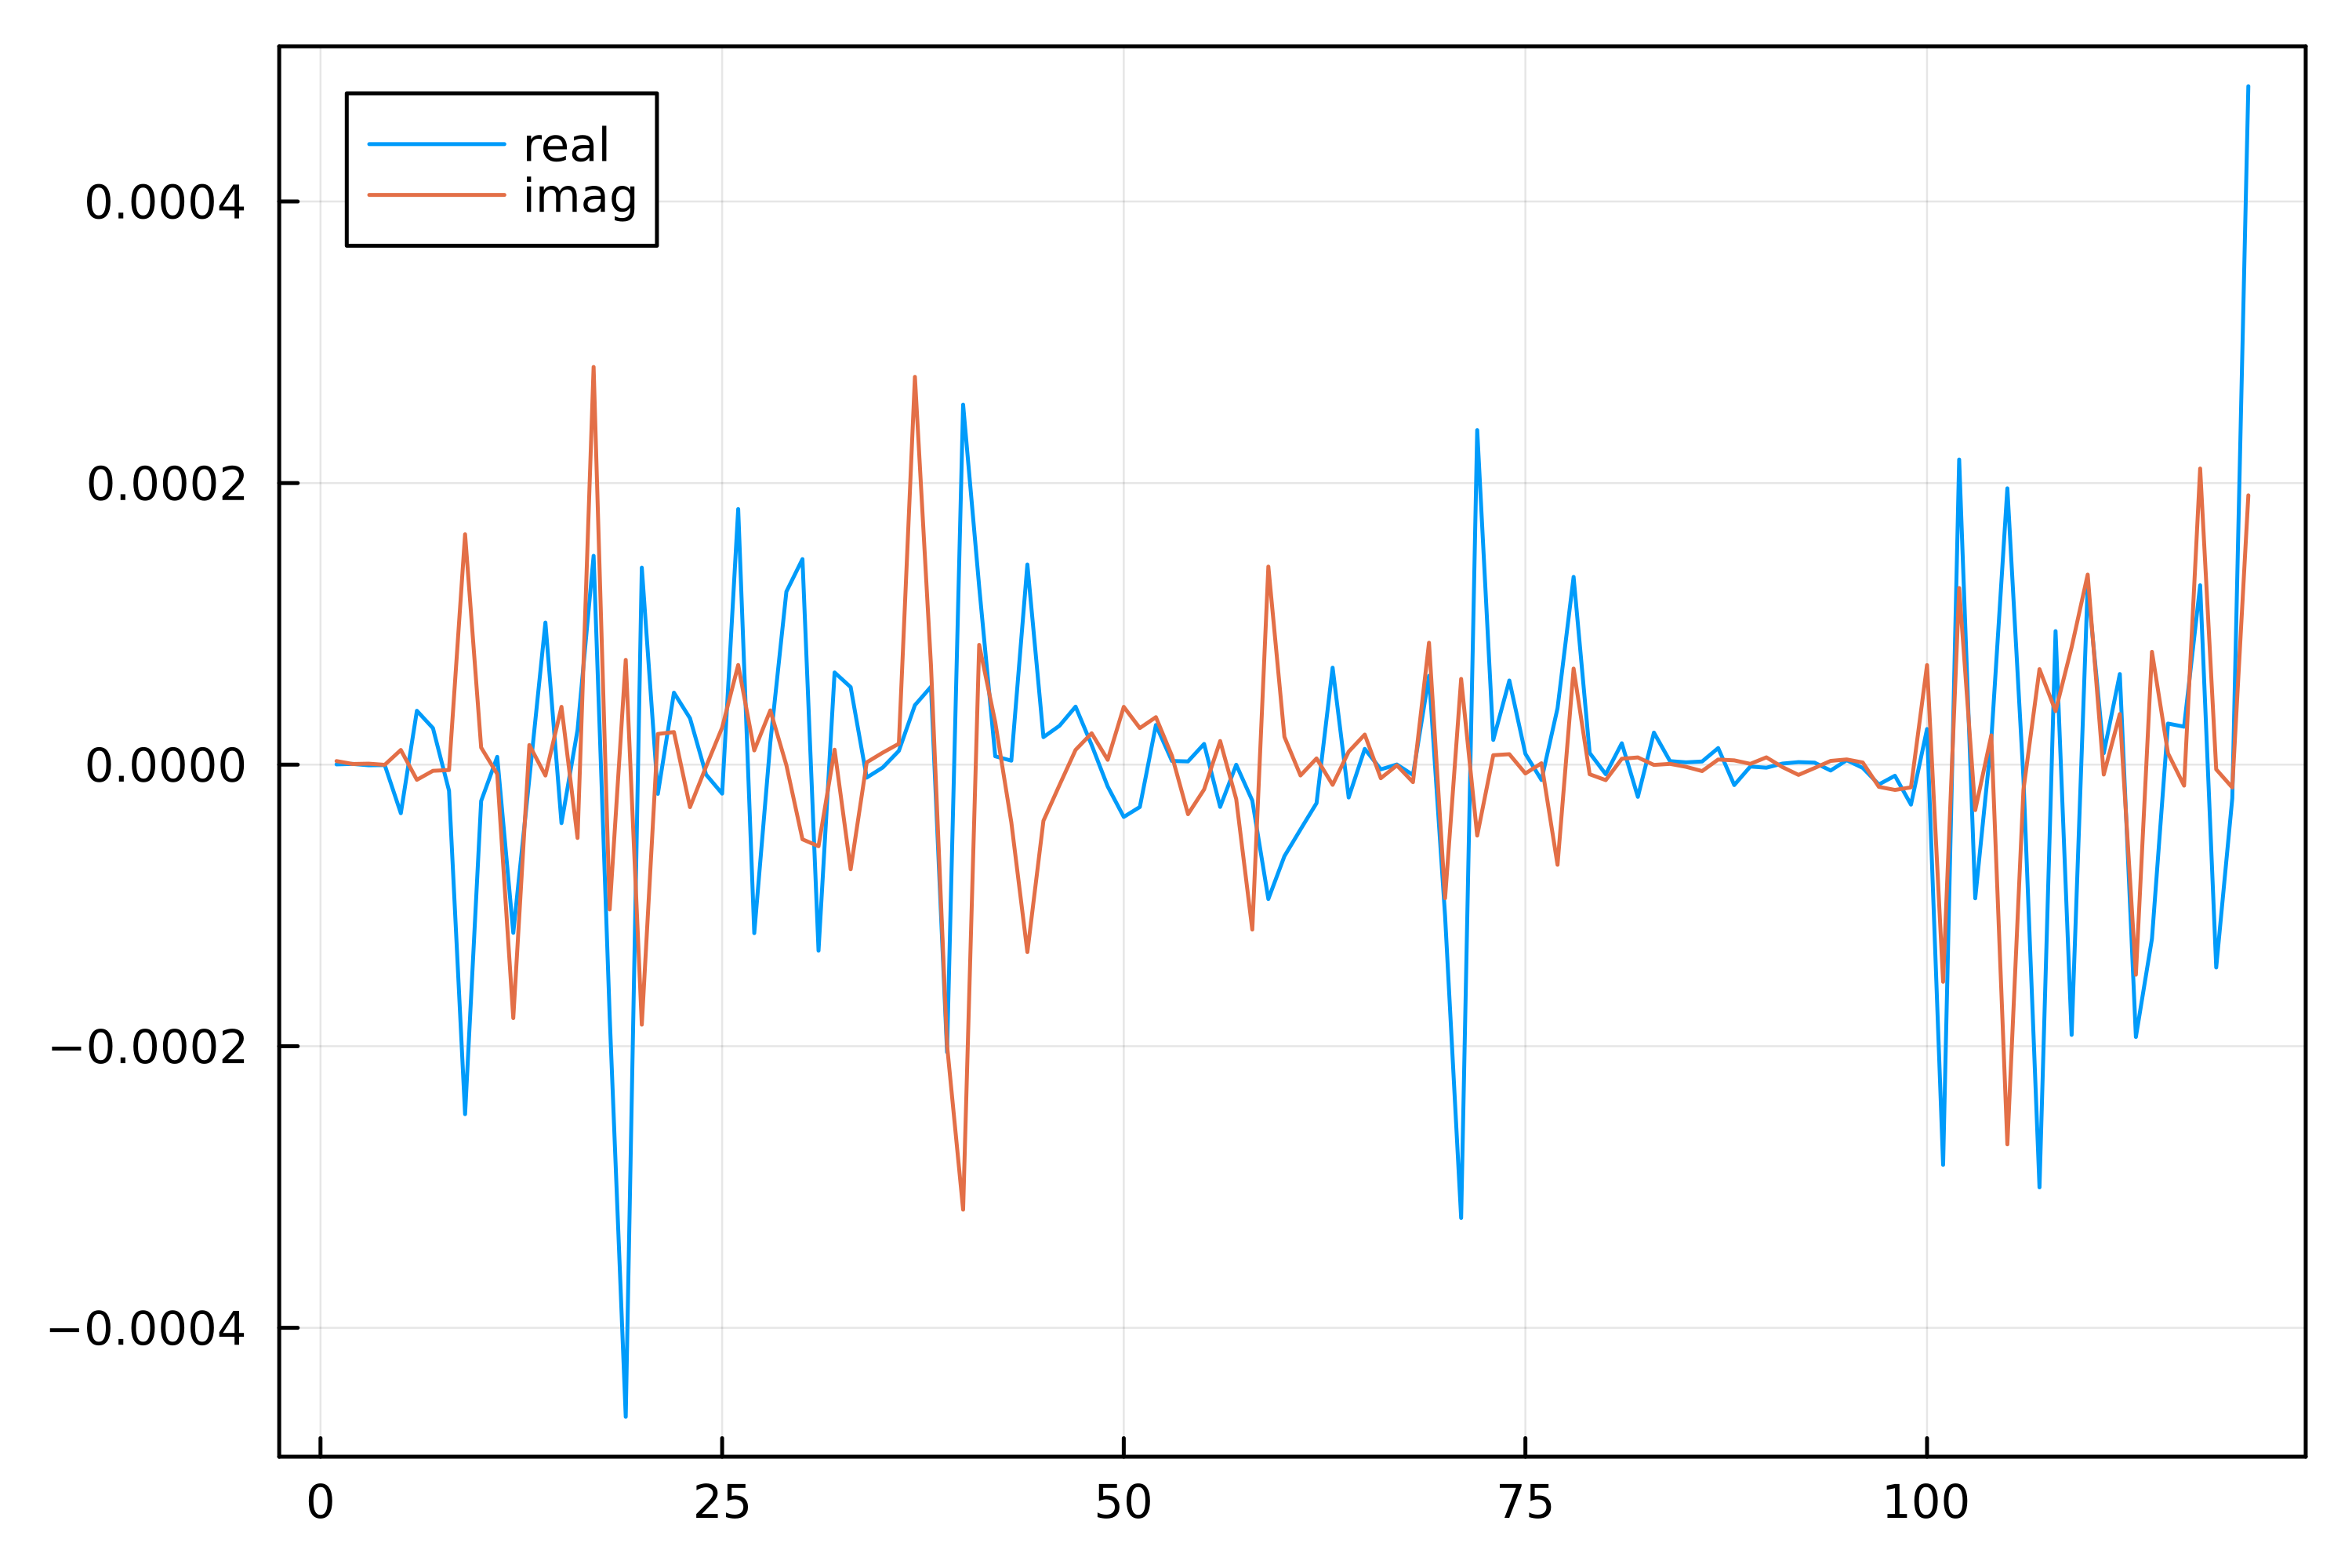
\includegraphics[width=\textwidth]{../data/chi/nc-n1-2000-n2-1000-nv-1-120-k_idx-12-q_idx-37-G_idx-200.png}
    \end{center}    
\end{column}

\begin{column}{0.4\textwidth}
    \faHandPointRight For a single $n$, $MM^*$ can be large;
    but they terms cancel each other $\Rightarrow$
    diagonal $\scriptstyle \sum_{n}^{\text{occ}} M_{n n'_1} (\vb{k}, \vb{q}, \vb{G}) M^*_{nn'_2} (\vb{k}, \vb{q}, \vb{G}')$
    
    \textbf{Why is this the case?}    
    
    \vspace{1cm}
    
    \faHandPointRight \textbf{The main reason: random phase factor in DFT diagonalization}
\end{column}

\end{columns}

\end{frame}

\begin{frame}
\frametitle{Cancellation of cross-terms in $\chi$}

\begin{columns}

\begin{column}{0.6\textwidth}
\small
\begin{equation*}
    \begin{aligned}
        &\quad \sum_{\vb{k}} \sum_{n}^{\text{occ}} M_{n n'_1}(\vb{k}, \vb{q}, \vb{G}) M_{n n'_2}^*(\vb{k}, \vb{q}, \vb{G}') \\
        &= \sum_{\vb{k}} \sum_{n}^{\text{occ}} \sum_{\vb{G}_1 \vb{G}_2} 
        c_{n \vb{k}+\vb{q}}^*(\vb{G} +\vb{G}_1)  c_{n_1' \vb{k}}(\vb{G}_1) 
        c_{n \vb{k}+\vb{q}}  (\vb{G}'+\vb{G}_2) c_{n_2' \vb{k}}^*(\vb{G}_2) \\
        \onslide<2->{
            &= \sum_{\vb{k}} \sum_{\vb{G}_1 \vb{G}_2} c_{n_1' \vb{k}}(\vb{G}_1) c_{n_2' \vb{k}}^*(\vb{G}_2)
            \textcolor[HTML]{4A90E2}{
                \underbrace{
                    \sum_{n}^{\text{occ}}  
                    c_{n \vb{k}+\vb{q}}^*(\vb{G}+\vb{G}_1) c_{n \vb{k}+\vb{q}}  (\vb{G}'+\vb{G}_2) 
                }_{\propto \delta_{\vb{G}_1 + \vb{G}, \vb{G}_2 + \vb{G}'} \text{ from approx. completeness}}            
            } \\
        }
        \onslide<3->{
            &\propto \sum_{\vb{G}_1} \sum_{\vb{k}} 
            \textcolor[HTML]{9013FE}{
                \underbrace{
                c_{n_1' \vb{k}}(\vb{G}_1) c_{n_2' \vb{k}}^*(\vb{G}_1 + \vb{G} - \vb{G}') 
                }_{\text{random phase cancellation}}
            } 
            \propto \delta_{n_1' n_2'}.
        }
    \end{aligned}
\end{equation*}
\normalsize
\end{column}

\begin{column}{0.35\textwidth} 
    \onslide<2->{
        \textcolor[HTML]{4A90E2}{In $\sum\limits_{n}^{\text{occ}}$: the number of $\vb{G}$ vectors making $c_{n \vb{k}}(\vb{G})$ non-zero 
        isn't much larger than $N_{\text{occ}}$: 
        we have an approximate, unnormalized completeness relation}
    }
    
    \vspace{1cm}

    \onslide<3->{
        \textcolor[HTML]{9013FE}{In $\sum_{\vb{k}}$: suppose $\theta_{n \vb{k}}$ is the random DFT diagonalization phase of $\ket*{\phi_{n \vb{k}}}$,
        $\sum_{\vb{k}} \ee^{\ii (\theta_{n_1' \vb{k}} - \theta_{n_2' \vb{k}})} \propto \delta_{n_1' n_2'}$}
    }
\end{column}

\end{columns}



\end{frame}

\section{\shortcode{pseudobands} for $\Sigma$}

\begin{frame}
\frametitle{$\Sigma^{\text{CH}}$ revisited}

Only $\Sigma^{\text{CH}}$ involves $\sum^{\text{emp}}$:
\scriptsize
\begin{equation*}
    \mel{n \vb{k}}{\Sigma^{\text{CH}}(\omega)}{n' \vb{k}} 
    = \frac{\ii}{2\pi} \sum_{n''} \sum_{\vb{q} \vb{G} \vb{G}'} 
    M^*_{n'' n} (\vb{k}, - \vb{q}, - \vb{G})  M_{n'' n'} (\vb{k}, - \vb{q},  -\vb{G}') 
    \int_{0}^{\infty} 
    \frac{
    [\epsilon^{\text{r}}(\vb{q}, \omega') - \epsilon^{\text{a}}(\vb{q}, \omega')]_{\vb{G} \vb{G}'}^{-1} 
    \dd{\omega'} 
    }{\omega - E_{n \vb{k}} - \omega' + \ii 0^+ \sgn(E_{n \vb{k}})} v(\vb{q}+\vb{G}')
    \label{eq:ch.simple}
\end{equation*}
\normalsize

\textbf{Problems} \begin{itemize}
    \item Summation over $\vb{G}$ very complicated $\Rightarrow$
    analysis based on $\vb{G}$ very hard.
    \item But at high empty bands, $\vb{G}'$ dominates $v(\vb{q} + \vb{G}')$ so the part besides $MM^*$ should be smooth w.r.t. $\vb{q}$
    \item and the summation over $\vb{q}$ still leads to the desirable diagonality 
\end{itemize}

-- But I don't have my own implementation of \shortcode{sigma} so that's pure speculation.

\end{frame}

\section{Enhancement of pseudobands: Felipe H. Jornada's recent paper}

\begin{frame}
\frametitle{``Stochastic'' pseudobands}

Energy averaging is also done in their paper:
\[
    G = \sum_{\text{$n$ near F.S.}} \frac{\dyad{\phi_{n \vb{k}}}}{\omega - E_{n \vb{k}}} + \sum_{\text{pseudobands block}} \frac{1}{\omega - \bar{E}} \sum_{n \in \text{block}} \dyad{\phi_{n \vb{k}}}.
\]     

\textbf{Their procedure} Replace each pseudobands block by \emph{several bands}:
\[
    \{\phi_{n \vb{k}}\}_{\text{$n$ in block}} \longrightarrow
    \left\{
        \ket*{\phi_{\xi \vb{k}}} = \sum_{\text{$n$ in block}} 
        \ee^{\ii \theta_{n \xi}} \ket*{\phi_{n \vb{k}}}
    \right\}_\xi
\]
\textbf{Justification} When $N_\xi \to \infty$, 
$\expval{
    \ee^{- \ii \theta_{n' \xi}} \ee^{\ii \theta_{n \xi}}
}_\xi = \delta_{n n'}$

\textbf{Comparison with the current script} When $N_\xi = 1$, 
$\ee^{\ii \theta_{n \xi}}$ comes from DFT diagonalization

\end{frame}

\begin{frame}
\frametitle{FHJ's justification of pseudobands}

\textbf{Convergence conditions} When $N_{\text{pseudobands blocks}} \to \infty$ and in each block $N_\xi \to \infty$, 
\begin{itemize}
    \item the expectations of $\chi$ and $\Sigma$ goes to the true value;
    \item the standard error goes to zero.
\end{itemize}

This convergence condition however is equivalent to not doing pseudobands at all\dots and their recommended values are not large enough anyway.

\uncover<2->{\textbf{They also realized this} ``the polarizability tends to converge much faster than $G$, partially due to the \emph{rapidly oscillating nature} of the matrix elements involving Kohn-Sham states used in the evaluation of the polarizability''

As is shown above.
}

\end{frame}

\begin{frame}
\frametitle{Compressing the bands even harder: size of blocks}

Recall that band dispersion is the main problem\dots

\[
    \begin{aligned}
        \Delta \chi \sim \frac{\Delta E}{E^2}, \quad \chi \sim \frac{1}{E} \Rightarrow
        \frac{\Delta \chi}{\chi} \simeq \frac{\Delta E}{E} \\
        \Rightarrow
        \frac{\Delta \chi}{\chi} \lesssim \const \Leftrightarrow \boxed{\frac{\Delta E}{E} \lesssim \const}
    \end{aligned}
\]

\textbf{Exponential growth of the energy spread of blocks!}

\end{frame}

\begin{frame}
\frametitle{Compressing the bands even harder: pseudobands near $E_{\text{F}}$?}

They claim that 
\begin{itemize}
    \item for \shortcode{epsilon}, bands near Fermi surface can also be pseudo-ized;
    \item for \shortcode{sigma}, only the bands near Fermi surface shouldn't be pseudo-ized.
\end{itemize}

\textbf{Important claim: protection window is not a convergence parameter: just protect a handful of bands and you're fine.} 


\emph{My own numerical experiments show that this is NOT the case when the band gap is very small so maybe a handful of bands still need to be protected.}

\end{frame}

\section{Discussion}

\begin{frame}
\frametitle{Discussion}
    
\textbf{Implications to $GW$ acceleration} There are lots of garbage in the giant input files we feed to $GW$

\textbf{Implications to machine learning} There exists an \emph{analytic} relation between $\epsilon^{\text{RPA}}, \Sigma^{GW}$ and $\{\bar{E}, \ket*{\phi_{\vb{k}}}^{\text{pseudo}} \}_{\text{blocks}}$

\begin{itemize}
    \item Pseudobands (with further compression of autoencoders) should be the starting point of all ML tasks
    \item Starting from pseudobands is \emph{not} feature engineering
\end{itemize}

\end{frame}

\end{document}